\chapter{分离变量法}
\thispagestyle{empty}
\section{预备知识}
\subsection{二阶线性常系数齐次微分方程}
\tdefination[特征根与与特征方程]
考虑方程
\begin{equation}
	y''+py'+qy=0
\end{equation}
其中,$p,q$是常数.考虑这个方程解的形式为
\begin{equation*}
	y=\e^{\lambda x}
\end{equation*}
代入原方程,消去$\e^{\lambda x}$则得到特征方程
\begin{equation}
	\lambda^2+p\lambda+q=0
\end{equation}
特征方程的根
\begin{equation}
	\lambda=\frac{1}{2}(-p\pm\sqrt{p^2-4q})
\end{equation}
称为特征根.
\jg

\theorem[二阶线性常系数齐次微分方程的通解]
\begin{table}[!htb]
	\centering
	\renewcommand{\arraystretch}{1}
	\setlength{\tabcolsep}{20mm}{
		\begin{tabular}{cc}
			\toprule[1.5pt] 
			特征根 &  通解形式 \\  
			\midrule
			两相异实根$\lambda_1,\lambda_2$& $\displaystyle C_1\e^{\lambda _1x}+C_2\e^{\lambda _2x}$\\
			二重根$\lambda_1$ & $\displaystyle (C_1+C_2x)\e^{\lambda _1x}$ \\
			共轭复根$\lambda_{1,2}=\alpha \pm \beta \rm{i}$& $\displaystyle \e^{\alpha x}(C_1\cos \beta x+C_2\sin \beta x)$ \\
			\bottomrule[1.5pt]
		\end{tabular}  
	}
	\caption{二阶线性常系数齐次微分方程的通解}
	\renewcommand{\arraystretch}{1}
	\label{二阶线性常系数齐次微分方程的通解}
\end{table} 

\subsection{函数的傅里叶级数展开}

\ttheorem[函数的正弦级数展开]
在$[0,l]$上定义的函数$f(x)$有正弦级数展开
\begin{equation}
	F(x) = \sum_{n = 1}^{\infty} b_n \sin \dfrac{n \pi}{l} x
\end{equation}
其中,
\begin{equation}
	b_n = \dfrac{2}{l} \int_{0}^{l} f(x)\sin \dfrac{n \pi}{l} x \,\d x
\end{equation}

\subsection{特征函数的正交性}

\ttheorem[特征函数的正交性]
设有一般形式的特征值问题
\begin{align*}
	X''(x) + \lambda X(x) = 0\\
	\alpha_1 X(0) + \beta_1 X'(0) = 0\\
	\alpha_2 X(0) + \beta_2 X'(0) = 0
\end{align*}
其中,$\alpha_1^2 + \beta_1^2 \neq 0, \alpha_2^2 + \beta_2^2 \neq 0.$

设$X_n$是对应特征值$\lambda_n$的特征函数,$X_m$是对应特征值$\lambda_m$的特征函数,且$m \neq n$,则特征函数的正交性的数学表达式为
\begin{align}
	\int_0^l X_n(x)X_m(x) \, \d x =0, \,\, n \neq m
\end{align}

\section{有界弦的自由振动}
\subsection{定解问题}
\noindent 方程
\begin{equation}
	\dfrac{\partial^2 u}{\partial t^2} = a^2 \dfrac{\partial^2 u}{\partial x^2}
	\label{定解1}
\end{equation}
边界条件
\begin{equation}
	\begin{cases}
		\left. u \right|_{x = 0} = 0\\
		\left. u \right|_{x = l} = 0
	\end{cases}
	\quad t > 0
\end{equation}
初始条件
\begin{equation}
	\begin{cases}
		\left. u \right|_{t = 0} = \varphi(x)\\[0.5em]
		\left. \dfrac{\partial u}{\partial t} \right|_{t = 0} = \psi(x)
	\end{cases}
\quad 0 \le x \le l
\end{equation}

\noindent 我们希望所求的解具有\dy[分离变量]{FLBL}的形式:
\begin{equation}
	u(x, t) = X(x)T(t)
\end{equation}

将方程\eqref{定解1}代入,可得
\begin{equation}
	X(x)T''(t)=a^2X''(x)T(t)
\end{equation}

\subsection{方程的处理}
由于我们求的是非零解,可以得到
\begin{equation}
	\dfrac{X''(x)}{X(x)} = \dfrac{1}{a^2}\dfrac{T''(t)}{T(t)}
\end{equation}
方程左端与$t$无关,右端与$x$无关,所以整个方程与$t,x$均无关,即为常数
\begin{equation}
	\dfrac{X''(x)}{X(x)} = \dfrac{1}{a^2}\dfrac{T''(t)}{T(t)} = -\lambda
\end{equation}
整理后得到
\begin{equation}
	\begin{cases}
		T''(t) + \lambda a^2 T(t)=0\\
		X''(x) + \lambda X(x) = 0
	\end{cases}
\end{equation}

\subsection{边界条件与初始条件的处理}
对于边界条件,可以得到
\begin{align*}
	\left. u \right|_{x = 0} = 0 \Rightarrow X(0)T(t) = 0 \Rightarrow X(0) = 0\\
	\left. u \right|_{x = l} = 0 \Rightarrow X(l)T(t) = 0 \Rightarrow X(l) = 0
\end{align*}
而对于初始条件,由于方程非齐次,不可以分离变量得到进一步的表达式。
\vspace*{0.5em}

\subsection{求解方程}
对于$X(x)$,我们得到二阶常微分方程
\begin{equation}
	\begin{cases}
		X''(x) + \lambda X(x) = 0\\
		X(0) = 0,\,\, X(l) = 0
	\end{cases}
\end{equation}
其特征方程为
\begin{equation}
	r^2 + \lambda = 0
\end{equation}
其特征根为
\begin{equation}
	r = \pm \sqrt{- \lambda}
\end{equation}
根据二阶线性常系数齐次微分方程对$\lambda$进行分类讨论求解:
\begin{enumerate}
	\item $\lambda = 0$
	\begin{itemize}
		\item 特征根为
		\begin{equation*}
			r_1 = r_2 = 0
		\end{equation*}
		\item 微分方程的通解为
		\begin{equation}
			X = Ax + B
		\end{equation}
	\item 由定解条件(边界条件),得到
	$
	\begin{cases}
		A = 0\\
		B = 0
	\end{cases}
	$
	\item 特解:$X = 0$
	\end{itemize}
\item $\lambda < 0$
\begin{itemize}
	\item 特征根为两个实根
	\begin{equation*}
		r_1 = \sqrt{- \lambda }, \quad  r_2 = -  \sqrt{- \lambda }
	\end{equation*}
	\item 微分方程的通解为
	\begin{equation}
		X = A\e^{r_1x}+B\e^{r_2x} = A\e^{\sqrt{- \lambda }x}+B\e^{-\sqrt{- \lambda }x} 
	\end{equation}
	\item 由定解条件(边界条件),得到
	$
	\begin{cases}
		A + B= 0\\
		A\e^{\sqrt{- \lambda }l}+B\e^{-\sqrt{- \lambda }l}  = 0
	\end{cases}
\Rightarrow A = B = 0
	$
	\item  特解:$X = 0$
\end{itemize}
\item $\lambda > 0 $
\begin{itemize}
	\item 特征根为一对共轭复数
	\begin{equation*}
		r_1 = \sqrt{\lambda}\i , r_2 = -\sqrt{\lambda} \i
	\end{equation*}
	\item 微分方程的通解为
	\begin{equation}
		X(x) = A \cos \sqrt{\lambda}x + B \sin \sqrt{\lambda}x
	\end{equation}
	\item 由定解条件(边界条件),得到$\begin{cases}
		A = 0\\
		B \sin \sqrt{\lambda} l = 0 
	\end{cases}$
.由于$B \neq 0$,所以$\sin \sqrt{\lambda} l =0$,即
\begin{align}
	\lambda = \left(\dfrac{n \pi}{l}\right)^2 = \dfrac{n^2 \pi^2}{l^2}
\end{align}
\end{itemize}
\end{enumerate}
所以,我们得到对应的解
\begin{align}
	\lambda_n = \left(\dfrac{n \pi}{l}\right)^2 = \dfrac{n^2 \pi^2}{l^2}\,\,(n =1, ,2,3, \cdots)\\[0.5em]
	X_n(x) = B_n \sin \dfrac{n \pi}{l}x \,\, (n = 1,2,3, \cdots )
\end{align}
其中$\lambda$只能取特定的值$\lambda_n$称为\dy[特征值]{TZZ},相应的非零解称为\dy[特征函数]{TZHS},求解$X(x)$的常微分问题称为\dy[特征值问题]{TZZWT}。


对于函数$T(t)$的常微分方程
\begin{equation*}
	T''(t) + \lambda a^2 T(t) = 0
\end{equation*}
由
\begin{equation*}
	\lambda_n = \dfrac{n^2 \pi^2}{l^2}, \quad n = 1,2,3,\cdots
\end{equation*}
得
\begin{equation*}
	T_n''(t) + \left(\dfrac{n\pi}{l}a\right)^2 T_n(t) = 0
\end{equation*}
由二阶线性常微分方程的解的形式可得
\begin{equation}
	T_n = C_n \cos \dfrac{n\pi}{l}at + D_n \sin \dfrac{n \pi }{l} a t
\end{equation}

因此,得到无穷多个线性无关且满足偏微分方程和边界条件的特解:
\begin{equation}
	u_n(x, t) = X_n(x)T_n(t)=\left(C_n \cos \dfrac{n \pi}{l}at + D_n \sin \dfrac{n \pi}{l} at \right)\sin \dfrac{n \pi}{l}x
\end{equation}
为满足初始条件,一般解为所有特解之和,即
\begin{align}
	u(x, t) = \sum_{n = 1}^{\infty} \left(C_n \cos \dfrac{n \pi}{l}at + D_n \sin \dfrac{n \pi}{l} at \right)\sin \dfrac{n \pi}{l}x
\end{align}
要求级数收敛,且能够对$x,t$逐项微分两次。

\subsection{代入初始条件}
由初始条件
\begin{equation*}
	\begin{cases}
		\left. u \right|_{t = 0} = \varphi(x)\\[0.5em]
		\left. \dfrac{\partial u}{\partial t} \right|_{t = 0} = \psi(x)
	\end{cases}
	\quad 0 \le x \le l
\end{equation*}
代入一般解,得到
\begin{equation*}
	\begin{cases}
		\displaystyle \sum_{n=1}^{\infty} C_n \sin \dfrac{n \pi}{l} x = \varphi(x)\\[1em]
		\displaystyle\sum_{n=1}^{\infty} D_n \dfrac{n \pi a}{l} \sin \dfrac{n \pi}{l} x = \psi(x)
	\end{cases}
\end{equation*}
由$\varphi(x),\psi(x)$的傅立叶级数,有
\begin{align}
	\varphi(x) = \sum_{n = 1}^{\infty} b_{1n} \sin \dfrac{n \pi}{l}x\\
	\psi(x) = \sum_{n=1}^{\infty} b_{2n} \sin \dfrac{n \pi}{l}x
\end{align}
即
\begin{align*}
	\displaystyle \sum_{n=1}^{\infty} C_n \sin \dfrac{n \pi}{l} x = \sum_{n = 1}^{\infty} b_{1n} \sin \dfrac{n \pi}{l}x \\[1em]
	\displaystyle \sum_{n=1}^{\infty} D_n \dfrac{n \pi a}{l} \sin \dfrac{n \pi}{l} x = \sum_{n = 1}^{\infty} b_{2n} \sin \dfrac{n \pi}{l}x
\end{align*}
比对系数可以得到
\begin{align*}
	C_n &= b_{1n} = \dfrac{2}{l} \int_{0}^{l} \left[\varphi(x) \sin \dfrac{n \pi}{l}x\right] \, \d x\\
	D_n &= \dfrac{l}{n \pi a} b_{2n} = \dfrac{2}{n \pi a}\int_{0}^{l} \left[\psi(x) \sin \dfrac{n \pi}{l}x\right] \, \d x
\end{align*}

\subsection{求解结果}
所以我们可以得到最终的方程解为
\begin{equation}
	u(x, t) = \sum_{n = 1}^{\infty} \left(C_n \cos \dfrac{n \pi}{l}at + D_n \sin \dfrac{n \pi}{l} at \right)\sin \dfrac{n \pi}{l}x
\end{equation}
其中
\begin{align}
	C_n &=  \dfrac{2}{l} \int_{0}^{l} \left[\varphi(x) \sin \dfrac{n \pi}{l}x\right] \, \d x\\[1em]
	D_n &=  \dfrac{2}{n \pi a}\int_{0}^{l} \left[\psi(x) \sin \dfrac{n \pi}{l}x\right] \, \d x
\end{align}

\subsection{分离变量法总结}
分离变量法的大致过程如图\ref{分离变量}.
\begin{figure}[!htb]
	\centering
	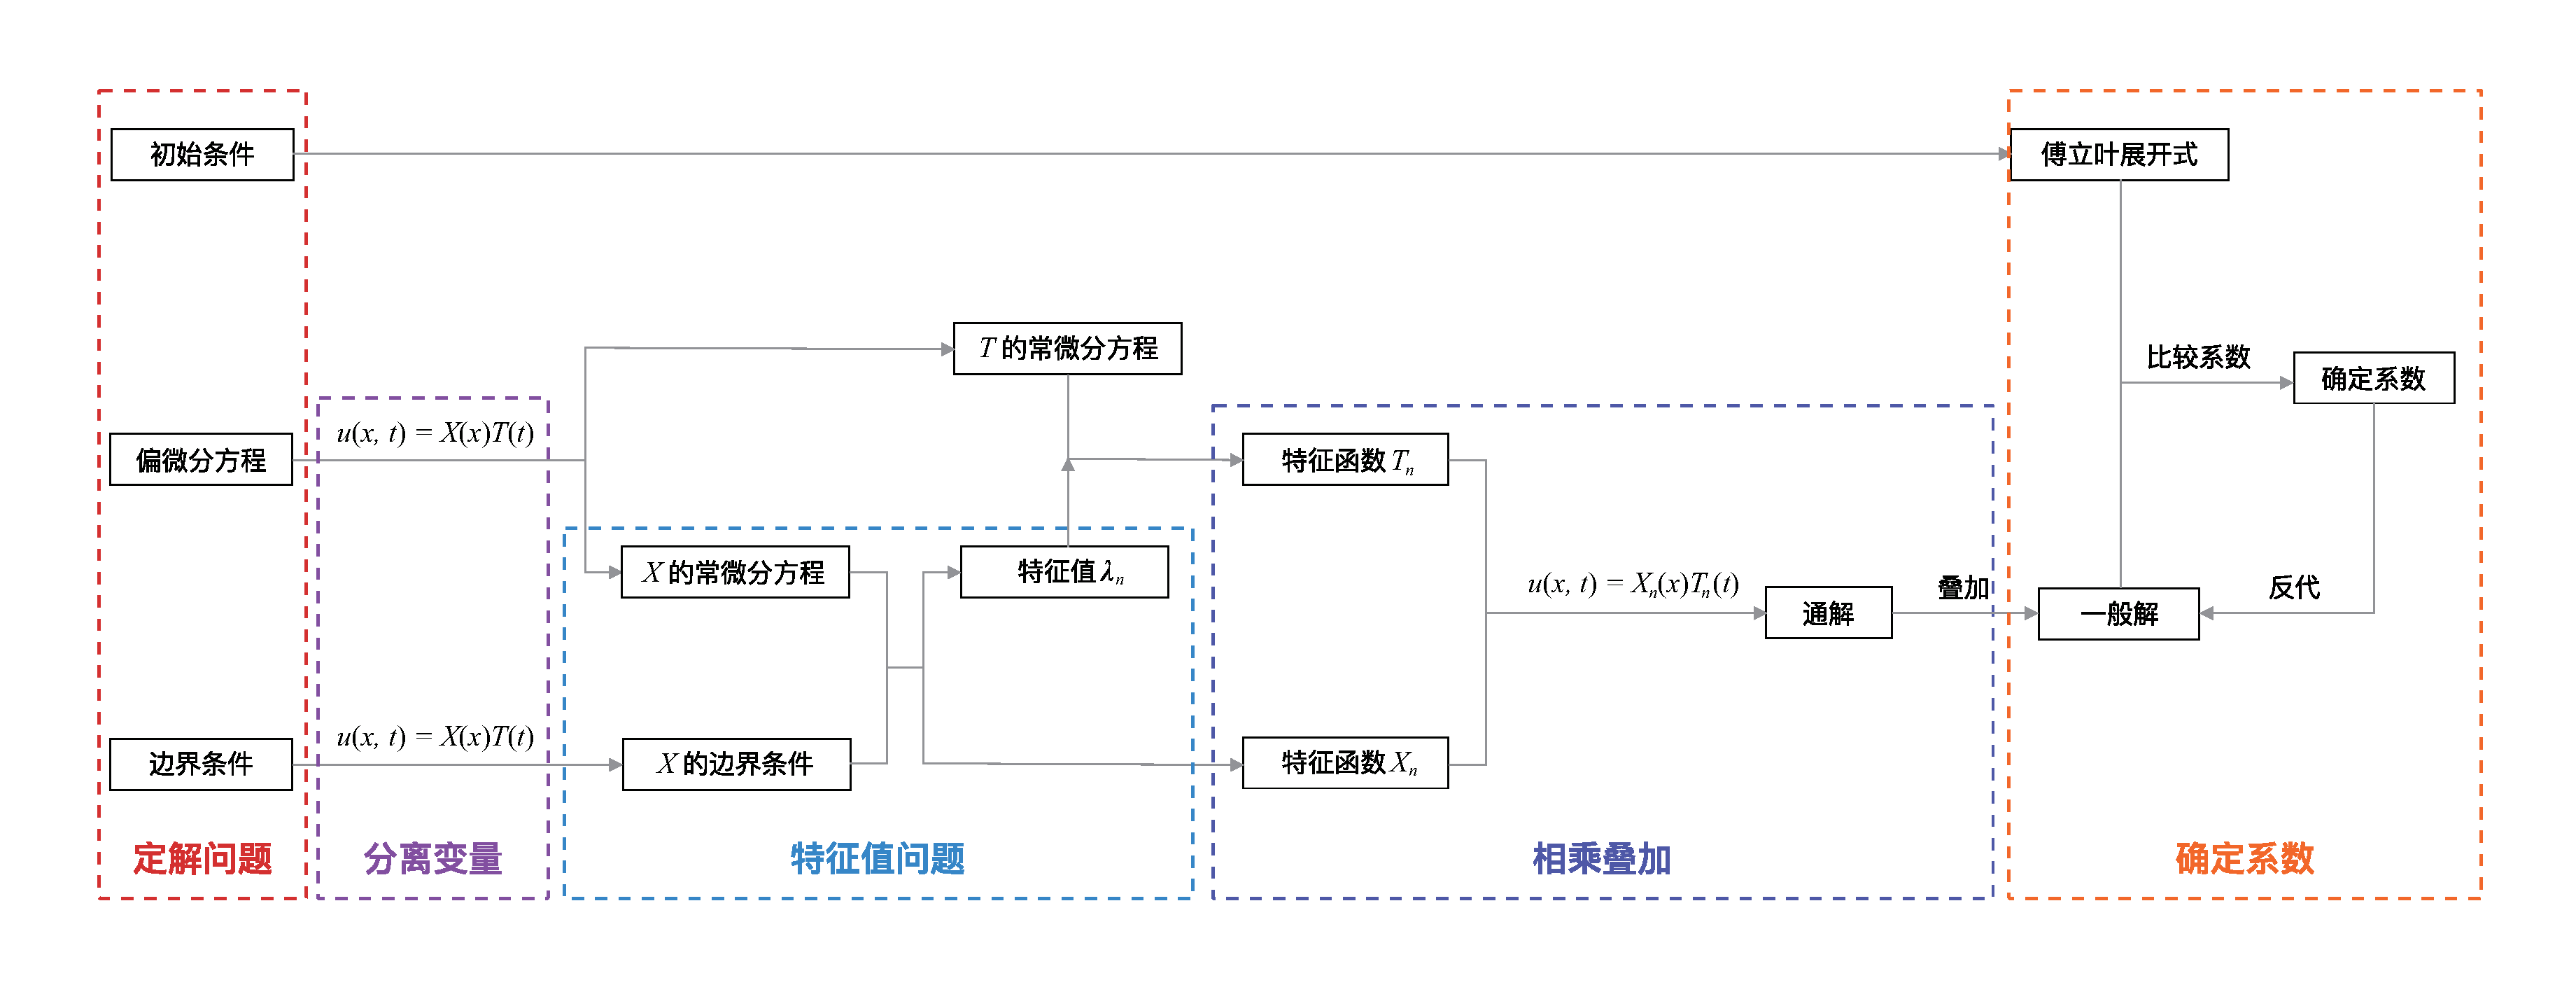
\includegraphics[width=\linewidth]{pic/分离变量.pdf}
	\caption{分离变量法总结}
	\label{分离变量}
\end{figure}

\section{有限杆的传热问题}
问题:设有一根长为$l$的均匀细杆,两端点为$x = 0$和$x = l$;在端点$x = 0$处温度为零摄氏度,而在另一端$x = l$处杆的热量自由散发到周围温度是零的介质中去,传热系数与杆导热系数之比为$h$。已知初始温度为$\varphi(x)$。求杆上的温度变化规律。

\subsection{定解问题}
方程
\begin{align}
	\dfrac{\partial u}{\partial t} = a^2 \dfrac{\partial^2 u}{\partial x^2}
\end{align}

边界条件\\
由牛顿冷却定律
\begin{align*}
	x= l: - k \dfrac{\partial u}{\partial x} = h(\left. u\right|_{x = l} - u_{\text{air}})=h\left. u\right|_{x = l}
\end{align*}
即
\begin{align}
	\left. u \right|_{x =0} = 0\\
	\left. \left(\dfrac{\partial u}{\partial x} + hu\right)\right|_{x = l} = 0
\end{align}

初始条件
\begin{align}
	\left. u \right|_{t = 0} = \varphi(x),\,\, 0 \le x \le l
\end{align}

\subsection{分离变量}
设$u(x, t) = X(x)T(t)$,分离方程,得
\begin{align*}
	 &X(x) T'(t) = a^2 T(t)X''(x)\quad  \Rightarrow \dfrac{1}{a^2} \dfrac{T'(t)}{T(t)} = \dfrac{X''(x)}{X(x)}
\end{align*}
由于$\dfrac{1}{a^2} \dfrac{T'(t)}{T(t)} $与$x$无关,$ \dfrac{X''(x)}{X(x)}$与$t$无关,所以
\begin{align}
	\dfrac{1}{a^2} \dfrac{T'(t)}{T(t)} = \dfrac{X''(x)}{X(x)} = - \lambda
\end{align}
即
\begin{align}
	X''(x) + \lambda X(x) = 0\\
	T'(t) + \lambda a^2 T(t) = 0
\end{align}

\subsection{特征值问题}
考虑边界条件
\begin{align*}
	\left. u \right|_{x =0} =0 \,\, \Rightarrow \,\, X(0)&T(t) = 0 \,\, \Rightarrow \, \, X(0) = 0\\
	\left. \left(\dfrac{\partial u}{\partial x} + hu\right)\right|_{x = l} = 0 \, \, \Rightarrow \,\, X'(l)T(t) &+ h X(l)T(t) = 0  \, \, \Rightarrow \,\,  X'(l) + hX(l) = 0
\end{align*}
那么得到常微分方程
\begin{align}
	\begin{cases}
		X''(x) + \lambda X(x) = 0\\
		X(0) = 0\\
		X'(l) + hX(l) = 0
	\end{cases}
\end{align}
其特征方程为
\begin{equation}
	r^2 + \lambda = 0
\end{equation}
其特征根为
\begin{equation}
	r = \pm \sqrt{- \lambda}
\end{equation}
对$\lambda$进行分类讨论
\begin{enumerate}
	\item $\lambda = 0$
	\begin{itemize}
		\item 特征根为
		\begin{equation*}
			r_1 = r_2 = 0
		\end{equation*}
		\item 微分方程的通解为
		\begin{equation}
			X = Ax + B
		\end{equation}
		\item 由定解条件(边界条件),得到
		$
		\begin{cases}
			B = 0\\
			A(1 + hl) + Bh = 0
		\end{cases}
		\quad \Rightarrow \quad
		\begin{cases}
			B = 0\\
			A = 0
		\end{cases}
		$
		\item 总方程:$X = 0$
	\end{itemize}
	
	\item $\lambda < 0$
	\begin{itemize}
		\item 特征根为两个实根
	\begin{equation*}
		r_1 = \sqrt{- \lambda }, \quad  r_2 = -  \sqrt{- \lambda }
	\end{equation*}
	\item 微分方程的通解为
	\begin{equation}
		X = A\e^{r_1x}+B\e^{r_2x} = A\e^{\sqrt{- \lambda }x}+B\e^{-\sqrt{- \lambda }x} 
	\end{equation}
	\item 由定解条件(边界条件),得到
	$
	\begin{cases}
		A + B= 0\\
		A(h + \sqrt{-\lambda})\e^{\sqrt{- \lambda }l} + B (h - \sqrt{- \lambda})\e^{-\sqrt{- \lambda }l}= 0
	\end{cases}
	\Rightarrow A(h + \sqrt{-\lambda})\e^{\sqrt{- \lambda }l} = A (h - \sqrt{- \lambda})\e^{-\sqrt{- \lambda }l}
	$
	\begin{itemize}
		\item 若$A \neq 0$\\
		两边同时除以$A$,得
		\begin{align*}
			(h + \sqrt{-\lambda})\e^{\sqrt{- \lambda }l} = (h - \sqrt{- \lambda})\e^{-\sqrt{- \lambda }l}\\
			\Longrightarrow \dfrac{h - \sqrt{-\lambda}}{h + \sqrt{- \lambda}} = \e^{2\sqrt{- \lambda }l}
		\end{align*}
	由于$\e^{2\sqrt{- \lambda }l} > 1$,而$\dfrac{h - \sqrt{-\lambda}}{h + \sqrt{- \lambda}} < 1$因此矛盾,故$A = 0$.
	\end{itemize}
	所以$A = B = 0$
	\item 总方程:$X = 0$
	\end{itemize}
	
	\item $\lambda > 0$
	\begin{itemize}
		\item 特征根为一对共轭复数
		\begin{equation*}
			r_1 = \sqrt{\lambda}\i , r_2 = -\sqrt{\lambda} \i
		\end{equation*}
		\item 微分方程的通解为
		\begin{equation}
			X(x) = A \cos \sqrt{\lambda}x + B \sin \sqrt{\lambda}x
		\end{equation}
		\item 由定解条件(边界条件),得到
		$\begin{cases}
			A\cos \sqrt{\lambda}l = 0 \rightarrow A = 0\\
			B\sqrt{\lambda}\cos \sqrt{\lambda}l + Bh \sin \sqrt{\lambda}l  = 0 
		\end{cases}$
		.由于$B \neq 0$,所以$\sqrt{\lambda}\cos \sqrt{\lambda}l + h\sin \sqrt{\lambda}l  = 0$,即
		\begin{align}
			\sqrt{\lambda} + h\tan \sqrt{\lambda}l =0 \Longrightarrow \sqrt{\lambda} = h\tan \sqrt{\lambda}l
		\end{align}
	\end{itemize}
\end{enumerate}
所以,我们得到
\begin{myitemize}
	\item 特征值为
	\begin{align}
		\sqrt{\lambda_n} = h\tan \sqrt{\lambda_n}l
	\end{align}
	\item 的解,特征函数为
	\begin{align}
		X_n(x) = B_n \sin \sqrt{\lambda_n}x
	\end{align}
\end{myitemize}
\vspace*{1em}

\subsection{相乘叠加得一般解}
将$\lambda_n$代入$T$的方程
\begin{align*}
	T_n'(t) + \lambda_n a^2 T_n(t) = 0
\end{align*}
解得
\begin{align}
	T_n = C'_n \e^{- \lambda_n a^2 t}
\end{align}

因此,得到无穷多个线性无关且满足偏微分方程和边界条件的特解:
\begin{equation}
	u_n(x, t) = X_n(x)T_n(t)=C_n \e^{- \lambda_n a^2 t} \sin \sqrt{\lambda_n}x
\end{equation}
为满足初始条件,令一般解为所有特解之和,即
\begin{align}
	u(x, t) = \sum_{n = 1}^{\infty} C_n \e^{- \lambda_n a^2 t} \sin \sqrt{\lambda_n}x
\end{align}
要求级数收敛,且能够对$x,t$逐项微分两次。

\subsection{确定叠加系数}
由初始条件
\begin{align*}
	u(x, 0) = \sum_{n = 1}^{\infty} C_n \sin \sqrt{\lambda_n} x = \varphi(x)
\end{align*}
由特征函数的正交性可得
\begin{align}
	\int_{0}^{l} X_m(x)X_n(x)\,\d x = 0, \,\, n \neq m\\
	\int_{0}^{l} \sin \sqrt{\lambda_m} x \sin \sqrt{\lambda_n} x \, \d x= 0, \,\, n \neq m
\end{align}
为了利用特征函数的正交性,两边同时乘以$\sin \sqrt{\lambda_m} x$再做积分,即
\begin{align}
	\int_{0}^{l} \left( \sum_{n= 1}^{\infty }C_n \sin \sqrt{\lambda_n} x \sin \sqrt{\lambda_m} x\right)\,\d x = \int_{0}^{l} \left[\varphi(x) \sin \sqrt{\lambda_m} x \right]\, \d x
\end{align}
逐项积分
\begin{align}
	\sum_{n= 1}^{\infty } \left[C_n \int_{0}^{l} \left(\sin \sqrt{\lambda_n}x \sin \sqrt{\lambda_m x} \right)\, \d x\right] =  \int_{0}^{l} \left[\varphi(x) \sin \sqrt{\lambda_m} x \right]\, \d x
\end{align}
由正交性质,得
\begin{align*}
	\sum_{n= 1}^{\infty } \left[C_n \int_{0}^{l} \left(\sin \sqrt{\lambda_n}x \sin \sqrt{\lambda_m x} \right)\, \d x\right] = C_m \int_{0}^{l} \left(\sin \sqrt{\lambda_m}x\right)^2 \, \d x
\end{align*}
即
\begin{align}
	C_n = \dfrac{\displaystyle \int_{0}^{l} \left[\varphi(x) \sin \sqrt{\lambda_n} x \right]\,\d x}{\displaystyle  \int_{0}^{l} \left(\sin \sqrt{\lambda_n}x\right)^2 \, \d x}
\end{align}

\section{非齐次方程的解法}
\subsection{特征函数展开法}
\noindent 将分离变量法进行改进,得到
\begin{enumerate}
	\item \textbf{求解特征值问题}
	$
	\begin{aligned}
		X''(x) &+ \lambda X(x) = 0\\
		&\mbox{边界条件}
	\end{aligned}
	$\\[0.5em]
	\textbf{获得特征函数族}$X_1(x),X_2(x), \cdots, X_n(x)$
	\item \textbf{直接将解写成特征函数族的展开式}
	\begin{align*}
		u(x, t) = \sum_{n = 1}^{\infty} u_n(x,t) = \sum_{n = 1}^{\infty } T_n(t)X_n(x)
	\end{align*}
	\item \textbf{代入方程,求解}$T_n(t)$.
\end{enumerate}

\subsection{两端固定弦的受迫振动}
\begin{enumerate}[\textbf{步骤}1\quad ]
	\item \textbf{一分为二}\\
	将弦的振动看作\textbf{初始条件引起的振动}和\textbf{强迫力引起振动}的叠加
	\begin{align*}
		\mbox{弦的振动}U(x,t)\,\,
		\begin{cases}
			\,\,\mbox{初始条件引起的振动} W(x,t)\\
			\,\, \mbox{强迫力引起的振动} V(x,t)
		\end{cases}
	\end{align*}
	于是将解作如下展开$U(x,t) = W(x,t)+ V(x,t)$
	\item \textbf{求解初始条件引起的振动}$W(x,t)$
	\begin{itemize}
		\item 列出定解问题
		\begin{align}
			\begin{cases}
				\,\dfrac{\partial^2 W}{\partial t^2} = a^2 \dfrac{\partial^2 W}{\partial t^2}, &0 < x < l, t>0\\
				\,\left. W \right|_{x= 0} = \left. W \right|_{x = l} = 0,& t> 0\\
				\,\left. W \right|_{t=0} = \varphi(x), \left. \dfrac{\partial W}{\partial t} \right|_{t = 0} = \psi(x),& 0 \le x \le l
			\end{cases}
		\end{align}
		\item 可以直接由前两节的分离变量法求得,这里不再赘述。
	\end{itemize}
	\item \textbf{求解强迫力引起的振动}$V(x,t)$
	\begin{itemize}
		\item 列出定解问题
		\begin{equation}
			\begin{cases}
				\,\dfrac{\partial^2 V}{\partial t^2} = a^2 \dfrac{\partial^2 V}{\partial x^2} + f(x,t), &0<x<l,t>0 \\[0.5em]
				\,\left. V \right|_{x = 0} = \left. V \right|_{x = l} = 0,& t>0\\[0.5em]
				\,\left. V \right|_{t = 0} = 0, \left. \dfrac{\partial V}{\partial t}\right|_{t = 0} = 0,& 0 \le x \le l
			\end{cases}
		\end{equation}
	\item 求解相应齐次方程的特征函数$X_n(x)$
		\begin{align}
			X''(x) + \lambda X(x) = 0
		\end{align}
	由前面几节的结果,可以得到
	\begin{align}
		X_n = B_n \sin \dfrac{n \pi}{l}x
	\end{align}
	\item 特征函数展开
	\begin{align}
		V(x, t) = \sum_{n = 1}^{\infty} v_n(t) X_n(x) = \sum_{n = 1}^{\infty} v_n(x)\sin \dfrac{n\pi}{l}x\\
		f(x,t) = \sum_{n = 1}^{\infty} f_n(t) X_n(x) = \sum_{n = 1}^{\infty} f_n(t)\sin \dfrac{n \pi}{l}x
	\end{align}
	\item 用特征函数正交性质求解$f_n(t)$
	\begin{align}
	 &\quad \quad f(x,t) = \sum_{n = 1}^{\infty} f_n(t) X_n(x) = \sum_{n = 1}^{\infty} f_n(t)\sin \dfrac{n \pi}{l}x \notag \\ 
	& \Rightarrow \int_{0}^l f(x,t) X_m(x) \,\d x = \sum_{n = 1}^\infty f_n(t) \int_0^l X_n(x)X_m(x)\, \d x = f_m(t) \int_0^l X^2_m(x)\, \d x \notag \\
	& \Rightarrow f_m(t) = \dfrac{\displaystyle \int_{0}^l f(x,t) X_m(x) \,\d x}{\displaystyle \int_0^l X^2_m(x)\, \d x} = \dfrac{2}{l} \int_0^l f(x,t) \sin \dfrac{m\pi}{l}x \,\d x
	\end{align}
	\item 将$V(x,t),f(x,t)$的展开式代入微分方程,得到关于$v_n(t)$的微分方程
	\begin{align*}
		\begin{aligned}
			V(x, t) = \sum_{n = 1}^{\infty} v_n(x)\sin \dfrac{n\pi}{l}x\\
			f(x,t) = \sum_{n = 1}^{\infty} f_n(t)\sin \dfrac{n \pi}{l}x
		\end{aligned}
		\quad \xrightarrow{\scriptsize \quad \mbox{代入}\quad }\quad 
		\dfrac{\partial^2 V}{\partial t^2} = a^2 \dfrac{\partial^2 V}{\partial x^2} + f(x,t)
	\end{align*}
	得到
	\begin{align}
		\sum_{n = 1}^\infty \left[v_n''(t) + \dfrac{a^2 n^2 \pi^2}{l^2}v_n(t) - f_n(t)\right] \sin\dfrac{n \pi}{l} \equiv 0
	\end{align}
	即
	\begin{align*}
		v_n''(t) + \dfrac{a^2 n^2 \pi^2}{l^2}v_n(t) = f_n(t)
	\end{align*}
	\item 将$V(x,t)$的展开式代入初始条件,得$v_n(t)$的初始条件
	\begin{align*}
		\left. V \right|_{t = 0} = 0 \quad \Rightarrow \quad v_n(0)X_n(x) = 0  \quad \Rightarrow \quad v_n(0) = 0\\
		\left. \dfrac{\partial V}{\partial t}\right|_{t = 0} = 0 \quad \Rightarrow \quad v_n'(0)X_n(x) = 0  \quad \Rightarrow \quad v_n'(0) = 0
	\end{align*}
	\item 求解$v_n(t)$的常微分方程
	\begin{align}
		\begin{cases}
			\,\, v_n''(t) + \dfrac{a^2 n^2 \pi^2}{l^2}v_n(t) = f_n(t)\\
			\,\, v_n(0) = 0, \,\, v_n'(0) = 0
		\end{cases}
	\end{align}
	由常数变易法或Laplace变换,得到
	\begin{align}
		v_n(t) = \dfrac{l}{n \pi a}\int_0^l f_n(\tau) \sin \dfrac{n \pi a (t - \tau)}{l}\, \d \tau 
	\end{align}
	\item 相乘叠加\\
	将计算结果代入特征函数的展开式,得到最终的结果
	\begin{align}
		V(x, t) = \sum_{n = 1}^\infty \left[\dfrac{l}{n \pi a}\int_0^l f_n(\tau) \sin \dfrac{n \pi a (t - \tau)}{l}\, \d \tau \right]\,\sin \dfrac{n \pi }{l}x
	\end{align}
	其中
	\begin{align*}
		f_n(t) = \dfrac{2}{l} \int_0^l f(x,t) \sin \dfrac{n\pi}{l}x \,\d x
	\end{align*}
	\end{itemize}

	\item \textbf{合二为一}\\
	两部分的结果叠加,得
	\begin{align}
		U(x,t) = W(x,t) + V(x, t)
	\end{align}
\end{enumerate}

总结如图\ref{非齐次方程求解总结图}.
\begin{figure}[!htb]
	\centering
	\begin{tikzpicture}
		\node (A) [draw, inner sep = 5pt]{求相应齐次问题的特征函数$X_n(x)$};
		\node (B) [draw, inner sep = 5pt, below of = A, node distance = 1.5cm]{解和非齐次项表示成特征函数的展开};
		\node (C1) [draw, inner sep = 5pt, below of = B, node distance = 3cm,xshift = -3.5cm]{$\displaystyle V(x,t) = \sum_{n = 1}^\infty v_n(t) X_n(x)$};
		\node (C2) [draw, inner sep = 5pt, below of = B, node distance = 3cm, xshift = 3.5cm]{$\displaystyle f(x,t) = \sum_{n = 1}^\infty f_n(t) X_n(x)$};
		\node (D2) [draw, inner sep = 5pt, below of = C2, node distance = 1.5cm]{根据特征函数正交性,获得系数$f_n(t)$};
		\node (E) [draw, inner sep = 5pt, below of = B, node distance = 6cm]{代入偏微分方程和初始条件,获得$v_n(t)$的常微分方程和定解条件};
		\node (F) [draw, inner sep = 5pt, below of = E, node distance = 1.5cm]{求解得$v_n(t)$,代回展开式得$V(x,t)$};
		
		\draw[arrows={-Stealth[scale=0.8]}] (A) -- (B);
		\draw[arrows={-Stealth[scale=0.8]}] (B) -- +(0cm, -1.5cm) -- +(-3.5cm,-1.5cm) -- (C1);
		\draw[arrows={-Stealth[scale=0.8]}] (B) -- +(0cm,-1.5cm) -- +(3.5cm,-1.5cm) -- (C2);
		\draw[arrows={-Stealth[scale=0.8]}] (C1) -- + (0cm, -2.25cm) -- +(3.5cm, -2.25cm) -- (E);
		\draw[arrows={-Stealth[scale=0.8]}] (C2) -- (D2);
		\draw[arrows={-Stealth[scale=0.8]}] (D2) -- +(0cm, -0.75cm) -- +(-3.5cm,-0.75cm) -- (E);
		\draw[arrows={-Stealth[scale=0.8]}] (E) -- (F);
	\end{tikzpicture}
\caption{非齐次方程求解总结图}
\label{非齐次方程求解总结图}
\end{figure}

\section{非齐次边界条件的处理}
\subsection{非齐次边界条件的概念}
前面所讨论的定解问题的解法, 不论方程是齐次的还是非齐次的,边界条件都是齐次的,由于非齐次边界条件不能分离变量,所以我们要将非齐次边界条件转换为齐次边界条件。

\subsection{非齐次边界条件的处理方法}
\begin{itemize}
	\item 总原则:设法将边界条件化成齐次的情况。
	\item 总思路:取一个适当的未知函数之间的代换,使对于新的未知函数,边界条件是齐次的。
\end{itemize}
\noindent 以定解问题为例
\begin{align}
	\begin{cases}
		\, \dfrac{\partial^2 u}{\partial t^2} = a^2 \dfrac{\partial^2 u}{\partial x^2} + f(x,t), 0<x<l,t>0 \\[0.5em]
		\, \left. u \right|_{x = 0} =u_1(t),  \left. u \right|_{x = l} = u_2(t), t>0\\[0.5em]
		\, \left. u \right|_{t = 0} = \varphi(x), \left. \dfrac{\partial u}{\partial t}\right|_{t = 0} = \psi(x), 0 \ge x \ge l
	\end{cases}
\end{align}
为使边界条件齐次化,作如下分解
\begin{align}
	u(x,t) = V(x,t) + W(x,t)
\end{align}
其中,令函数$W(x,t)$满足$u(x, t)$的边界条件
\begin{align}
	\left. W \right|_{x = 0} = u_1(t),\quad \left. W \right|_{x = l} = u_2(t)
	\label{边界条件}
\end{align}
则函数$V(x,t)$的边界条件是齐次的
\begin{align*}
	\left. V \right|_{x = 0}, \quad \left. V \right|_{x = l} = 0
\end{align*}
由于$W(x,t)$是满足条件\eqref{边界条件}的表达式,简单起见,设
\begin{align}
	W(x,t)= A(t)X + B(t)
\end{align}
即得到
\begin{align*}
	\begin{cases}
		\, W(0,t) = B(t) = u_1(t)\\
		\, W(l ,t) = A(t) l + B(t) = u_2 (t)
	\end{cases}
\quad \Longrightarrow \quad
\begin{cases}
	\, A(t) = \dfrac{u_2(t) - u_1(t)}{l}\\
	\, B(t) = u_1(t)
\end{cases}
\end{align*}
所以
\begin{align}
		W(x,t)= \dfrac{u_2(t) - u_1(t)}{l}x + u_1(t)
\end{align}
于是我们作以下变换
\begin{align}
	u(x,t) = V(x,t) +  \dfrac{u_2(t) - u_1(t)}{l}x + u_1(t)
\end{align}
得到转换后的定解问题
\begin{align}
	&\dfrac{\partial^2 V}{\partial t^2} = a^2 \dfrac{\partial^2 V}{\partial x^2} + F(x,t), 0<x<l,t>0\notag \\[0.5em]
	& \left. V \right|_{x = 0} =0,  \left. V \right|_{x = l} = 0, t>0\\[0.5em]
	& \left. V \right|_{t = 0} = \varPhi(x), \left. \dfrac{\partial V}{\partial t}\right|_{t = 0} = \varPsi(x), 0 \le x \le l\notag
\end{align}
其中
\begin{align*}
	F(x,t) &= f(x,t) - \left[\dfrac{u_2''(t) - u_1''(t)}{l}x + u_1''(t) \right]\\[0.5em]
	\varPhi(x) &= \varphi(x) - \left[\dfrac{u_2(t) - u_1(t)}{l}x + u_1(t)  \right]\\[0.5em]
	\varPsi (x) &= \psi (x) - \left[\dfrac{u_2(t) - u_1(t)}{l}x + u_1(t) \right]
\end{align*}

\subsection{四类非齐次边界条件的齐次化函数}
\begin{table}[!htb]
	\centering
	\renewcommand{\arraystretch}{1}
	\setlength{\tabcolsep}{12mm}{
		\begin{tabular}{cc}
			\toprule[1.5pt] 
			 边界条件 &  齐次化函数$W(x)$ \\  
			\midrule
			& \vspace*{-1em}\\
			$ \left. u \right|_{x = 0} =u_1(t),  \left. u \right|_{x = l} = u_2(t)$& $W(x,t)= \dfrac{u_2(t) - u_1(t)}{l}x + u_1(t)$\\
			& \vspace*{-1em}\\
			\hline
			& \vspace*{-1em}\\
			$u|_{x = 0} = u_1(t), \left. \dfrac{\partial u}{\partial x}\right|_{x = l} = u_2(t)$ & $\displaystyle W(x,t)= u_1(t)x + u_2(t)$ \\
			& \vspace*{-1em}\\
			\hline
			& \vspace*{-1em}\\
			$\left. \dfrac{\partial u}{\partial x}\right|_{x = 0} = u_1(t), u|_{x = l} = u_2(t)$& $\displaystyle W(x,t)= u_2(t)x + u_2(t) - lu_1(t)$ \\
			& \vspace*{-1em}\\
			\hline
			& \vspace*{-1em}\\
			$\left. \dfrac{\partial u}{\partial x}\right|_{x = 0} = u_1(t), \left. \dfrac{\partial u}{\partial x}\right|_{x = l} = u_2(t)$& $\displaystyle W(x,t)= \dfrac{u_2(t) - u_1(t)}{2l}x^2 + u_1(t)x$ \\
			& \vspace*{-1em}\\
			\bottomrule[1.5pt]
		\end{tabular}  
	}
	\caption{四类非齐次边界条件的齐次化函数}
	\renewcommand{\arraystretch}{1}
	\label{四类非齐次边界条件的齐次化函数}
\end{table} 
\vspace*{-2em}

\warn[
\begin{itemize}
	\item 选取不同的齐次化函数$W(x,t)$,导出的$V(x,t)$的定解问题也就不同,求出的$V(x,t)$也就不同
	\item 但\textbf{定解问题的解的存在唯一性},保证了最后解得的$u(x,t)$一定是相同的,尽管表达式的形式可能有所不同
	\item $W(x,t)$的选取原则是使自己的表达式尽可能简单的同时,也尽量使$V(x,t)$的定解问题尽可能简单
\end{itemize}
]

\subsection{方程和边界条件同时齐次化的情形}
最理想的情况是,不论原来的方程$u(x,t)$是不是齐次的,最终$V(x,t)$的方程是齐次的,即\textbf{方程和边界条件同时齐次化}。

\textbf{所需要的条件:当$u(x,t)$定解问题中的非齐次项、边界条件都与时间$t$无关。}

\examples 齐次化下列定解问题
\begin{align*}
	\begin{cases}
		\,\, \dfrac{\partial u}{\partial t} = a^2 \dfrac{\partial^2 u}{\partial x^2} + x^2, 0<x<l, t>0,\\
		\,\, u|_{x = 0} = A, \,\, u|_{x=l} = B, t>0, \\
		\,\, u|_{t = 0} = g(x), 0 \le x \le l
	\end{cases}
\end{align*}
\solve
设$u(x,t) = v(x,t) + w(x)$,$w(x)$满足边界条件,即
\begin{align}
	w(0) = A\\
	w(l) = B
\end{align}
将$u(x,t) = v(x,t) + w(x)$代入偏微分方程,得
\begin{align*}
	v_t = a^2(v_{xx} + w''(x)) + x^2 \Rightarrow v_t = a^2v_{xx} + a^2w''(x) + x^2
\end{align*}
为了使该偏微分方程是齐次的,则满足
\begin{align}
	w''(x) = - \dfrac{x^2}{a^2}
\end{align}
则得到$w(x)$的常微分方程
\begin{align}
	\begin{cases}
		\,\, w''(x) = - \dfrac{x^2}{a^2}\\
		\,\, w(0) = A\\
		\,\, w(l) = B
	\end{cases}
\end{align}
首先求得通解为
\begin{align}
	w(x) = -\dfrac{1}{12a^2}x^4 + C_1x + C_2
\end{align}
代入定解条件,得
\begin{align*}
	\begin{cases}
		\,\, C_2 = A\\
		\,\, -\dfrac{1}{12a^2}l^4 + C_1 l +C_2 = B
	\end{cases}
	\quad 
	\Rightarrow
	\quad 
	\begin{cases}
		\,\, C_2 = A\\
		\,\,  C_1 = \dfrac{B-A}{l}+\dfrac{l^3}{12a^2}
	\end{cases}
\end{align*}
所以
\begin{align}
	w(x) = \dfrac{1}{12a^2}x^4 + \left(\dfrac{B-A}{l}+\dfrac{l^3}{12a^2} \right)x + A
\end{align}
初始条件变为
\begin{align*}
	u|_{t = 0} = v(x, 0) + w(x) = g(x) \Rightarrow v(x,0) = g(x) - w(x) = g(x) -  \dfrac{1}{12a^2}x^4 - \left(\dfrac{B-A}{l}+\dfrac{l^3}{12a^2} \right)x - A
\end{align*}
所以齐次化后的定解问题为
\begin{align}
	\begin{cases}
		\,\, \dfrac{\partial v}{\partial t} = a^2 \dfrac{\partial^2 v}{\partial x^2}, 0<x<l, t>0,\\
		\,\, u|_{x = 0} = 0, \,\, u|_{x=l} = 0, t>0, \\
		\,\, v|_{t = 0} = g(x) -  \dfrac{1}{12a^2}x^4 - \left(\dfrac{B-A}{l}+\dfrac{l^3}{12a^2} \right)x - A, 0 \le x \le l
	\end{cases}
\end{align}


\section{圆域内的二维Laplace方程的稳定问题}
\subsection{预备知识}
\noindent \textbf{1.极坐标系下的Laplace方程}

直角坐标下的Laplace方程为
\begin{align}
	\dfrac{\partial^2 u}{\partial x^2} + \dfrac{\partial^2 u}{\partial y^2} = 0
\end{align}
极坐标与直角坐标的关系为
\begin{align}
	\begin{cases}
		\, x = r\cos \theta \\
		\, y = r \sin \theta 
	\end{cases}
\end{align}
由链式求导法则,得到极坐标下的Laplace方程为
\begin{align}
	\dfrac{\partial^2 u}{\partial r^2} + \dfrac{1}{r}\dfrac{\partial u}{\partial r} + \dfrac{1}{r^2}\dfrac{\partial^2 u}{\partial \theta^2} = 0\\[1em]
	\dfrac{1}{r}\dfrac{\partial}{\partial r}\left(r \dfrac{\partial u}{\partial r}\right)+\dfrac{1}{r^2}\dfrac{\partial^2 u}{\partial \theta^2} =0
\end{align}
特点:
\begin{itemize}
	\item 由于$r = 0$处导数不存在,不满足方程,所以\textbf{需要在$r=0$处补充边界条件};
	\item 周期性:$u|_{\theta} = u|_{\theta + 2 \pi}$
\end{itemize}

\noindent \textbf{2.以$2 \pi$为周期的函数傅立叶级数展开}
\begin{align}
	f(\theta) = \dfrac{A_0}{2}+ \sum_{n = 1}^{\infty} A_n\cos n\theta +B_n \sin n\theta
\end{align}
其中
\begin{align*}
	A_n &= \dfrac{1}{\pi} \int_{0}^{2\pi}f(\theta)\cos n\theta \, \d \theta,\quad n = 0,1,2,\cdots\\[1em]
	B_n &= \dfrac{1}{\pi} \int_{0}^{2\pi}f(\theta)\sin n\theta \, \d \theta,\quad n = 1,2,\cdots
\end{align*}

\subsection{物理问题}
一个半径为$r_0$的薄圆盘,上下两面绝热,圆周边缘温度已知,求达到温恒状态时圆盘内的温度分布。
\begin{enumerate}[\textbf{步骤}1 ]
	\item \textbf{列出定解问题}
	\begin{align}
		\begin{cases}
			\, \dfrac{\partial^2 u}{\partial x^2} + \dfrac{\partial^2 u}{\partial y^2} = 0, \,\, x^2 + y^2 \le r_0^2 \\[0.5em]
			\, u|_{x^2 + y^2 = r_0^2} = f(x,y)
		\end{cases}
	\end{align}
	\item \textbf{换成极坐标形式}\\
	换成极坐标的过程中,由于$r = 0$处导数不存在。因此,为了满足方程的适定性,需要补充$r = 0$处的边界条件。
	
	由于$r = 0$处没有热源且绝热,所以$r=0$处的温度不可能趋于无穷大,即
	\begin{align*}
		\left|u|_{r = 0}\right| < + \infty
	\end{align*}
	所以,最终形式的定解问题为
	\begin{align}
		\begin{cases}
			\, \dfrac{1}{r}\dfrac{\partial}{\partial r}\left(r \dfrac{\partial u}{\partial r}\right)+\dfrac{1}{r^2}\dfrac{\partial^2 u}{\partial \theta^2} =0, \,\, 0<r<r_0, -\infty < \theta < + \infty\\[0.5em]
			\, u|_{r = r_0} = f(\theta),\\
			\, \left|u|_{r = 0}\right| < + \infty,\\
			\, u|_{\theta} = u|_{\theta + 2\pi}
		\end{cases}
	\end{align}

	\item \textbf{分离变量}\\
	设$u(r,\theta) = R(r) \Phi(\theta)$,代入偏微分方程,得
	\begin{align*}
		& \,\,\,\,\, r^2 R''(r)\Phi(\theta) + r R'(r)\Phi(\theta) +R(r) \Phi''(\theta) = 0\\
		\Rightarrow & \,\,\,\, \Phi(\theta)\left[r^2 R''(r) + rR'(r)\right] = R(r)\Phi(\theta)\\
		\Rightarrow & \,\,\,\, -\dfrac{r^2 R''(r) + rR'(r)}{R(r)}=\dfrac{\Phi''(\theta)}{\Phi(\theta)}
	\end{align*}
	由于方程左边是关于$r$的函数,方程右边是关于$\theta$的函数,所以
	\begin{align*}
		-\dfrac{r^2 R''(r) + rR'(r)}{R(r)}=\dfrac{\Phi''(\theta)}{\Phi(\theta)} = -\lambda
	\end{align*}
	从而得到两个常微分方程
	\begin{align*}
		\begin{cases}
			\, \Phi''(\theta) + \lambda \Phi(\theta) = 0\\
			\, r^2 R''(r) + rR'(r) - \lambda R(r) = 0
		\end{cases}
	\end{align*}
	对于初始条件,由于$u|_{r =r_0} = f(\theta)$是非齐次的,而$\big|u|_{r = 0}\big|<+\infty$是有界条件,都不能分离变量。所以,我们尝试对周期性条件进行分离变量
	\begin{align*}
		R(r) \Phi(\theta) = R(r) \Phi(\theta + 2\pi) \quad \Rightarrow \quad \Phi(\theta) = \Phi(\theta + 2\pi) 
	\end{align*}
	
	\item \textbf{求解特征值问题}\\
	我们得到关于$\Phi(\theta)$的定解常微分方程
	\begin{align}
		\begin{cases}
			\, \Phi''(\theta) + \lambda \Phi(\theta) = 0\\
			\, \Phi(\theta) = \Phi(\theta + 2\pi)
		\end{cases}
	\end{align}
	对$\lambda$进行分类讨论
	\begin{itemize}
		\item $\lambda = 0$
		\begin{itemize}
			\item 通解\quad $\Phi''(\theta) =0 \quad \Rightarrow \quad \Phi(\theta) = A \theta + B$
			\item 特解 \quad $\Phi(\theta) = \Phi(\theta + 2\pi) \quad \Rightarrow \quad \Phi(\theta) = B$
		\end{itemize}
		所以$\lambda = 0$是特征值,$\Phi(\theta) = B$
	
		\item $\lambda < 0$
		\begin{itemize}
			\item 通解\quad $\Phi(\theta) = A\e^{\sqrt{-\lambda}\theta} + B \e^{-\sqrt{-\lambda}\theta}$
			\item 特解 \quad 由于实数域内指数函数不是周期函数,所以$A = B = 0$,舍去
		\end{itemize}
		
		\item $\lambda > 0$
		\begin{itemize}
			\item 通解\quad $\Phi(\theta) = A \cos \sqrt{\lambda}\theta  + B\sin \sqrt{\lambda}\theta $
			\item 特解 \quad $\Phi(\theta) = A \cos \sqrt{\lambda}\theta  + B\sin  \sqrt{\lambda}\theta $ 的周期为$\dfrac{2 \pi}{\sqrt{\lambda}}$,由于$\Phi(\theta)$是以$2 \pi $为周期的函数,则
			\begin{align*}
				\dfrac{2 \pi}{\sqrt{\lambda}} = \dfrac{2\pi}{n}, \,\, n = 1,2,3,\cdots
			\end{align*}
			即
			\begin{align}
				&\lambda_n = n^2\\
				&\Phi_n(\theta) = A_n \cos n\theta  + B_n \sin n\theta 
			\end{align}
		\end{itemize}
	\end{itemize}
	所以,特征值为
	\begin{align*}
		\begin{cases}
			\, \lambda_0 = 0,\,\, \Phi_0(\theta) = B_0\\
			\, \lambda_n = n^2,\, \, \Phi_n(\theta) = A_n \cos n\theta  + B_n \sin n \theta ,\,\, n = 1,2,3,\cdots
		\end{cases}
	\end{align*}

	\item \textbf{解另一方程}\\
	对关于$R(r)$的微分方程进行变形
	\begin{align*}
		&\,\,\quad r^2 R''(r) + rR'(r) - \lambda R(r) = 0\\
		\Rightarrow & \,\quad r \dfrac{\d }{\d r}\left(r \dfrac{\d R}{\d r}\right) - \lambda R = 0\\
		\Rightarrow & \,\quad \dfrac{\d }{\d \ln r} \left(\dfrac{\d R}{\d \ln r}\right) - \lambda R = 0
	\end{align*}
	\begin{itemize}
		\item $\lambda = 0 \quad \Rightarrow \quad \dfrac{\d }{\d \ln r} \left(\dfrac{\d R}{\d \ln r}\right) = 0 \quad \Rightarrow \quad R_0(r) = C_0 + D_0 \ln r$\vspace*{1em}
		
		\item $\lambda = n^2 \quad \Rightarrow \quad \dfrac{\d }{\d \ln r} \left(\dfrac{\d R}{\d \ln r}\right) - n^2 R = 0 \quad \Rightarrow \quad R_n(r) = C_n \e^{n \ln r} + D_n \e^{-n \ln r} = C_n r^n + D_n r^{-n}$
	\end{itemize}

	\item \textbf{相乘得特解}
	\begin{align*}
		\begin{cases}
			\, R_0(r) = C_0 + D_0 \ln r\\
			\, \Phi(\theta) = B_0\\
		\end{cases}
	\quad \Rightarrow \quad u(r, \theta) = B_0(C_0 + D_0 \ln r)
	\end{align*}
	\vspace*{-1.5em}
	\begin{align*}
		\begin{cases}
			\, R_n(r) = C_n r^n + D_n r^{-n}\\
			\, \Phi_n(\theta) = A_n \cos(n\theta) + B_n \sin(n \theta)\\
		\end{cases}
		\quad \Rightarrow \quad u(r, \theta) = \big(C_n r^n + D_n r^{-n}\big)\big(A_n \cos(n\theta) + B_n \sin(n \theta)\big)
	\end{align*}
	
	\item \textbf{叠加得一般解}
	\begin{align}
		u(r, \theta) =  B_0(C_0 + D_0 \ln r) + \sum_{n = 1}^\infty \big(C_n r^n + D_n r^{-n}\big)\big(A_n \cos n\theta + B_n \sin n \theta \big)
	\end{align}

	\item \textbf{确定叠加系数}\\
	仍有两个非齐次边界条件未使用,用它们来确定叠加系数。即叠加系数的确定,是要\textbf{满足非齐次边界条件},这与求解波动方程和热传导方程不同。
	\begin{itemize}
		\item 根据$r = 0$处$u$的有界性$\left|u|_{r = 0}\right| < + \infty$,结合一般解,发现两个发散量
		\begin{align*}
			\lim\limits_{r \to 0} \ln r &= - \infty\\
			\lim\limits_{r \to 0,\,\, n\to \infty} r^{-n} &= + \infty
		\end{align*}
		所以它们所对应的系数为0,即$D_0, D_n = 0$,一般解化简为
		\begin{align*}
			u(r, \theta) =  B_0C_0 + \sum_{n = 1}^\infty C_n r^n (A_n \cos n\theta + B_n \sin n \theta)
		\end{align*}
		
		\item 将一般解写成如下形式
		\begin{align}
			u(r, \theta) =  \dfrac{a_0}{2} + \sum_{n = 1}^\infty  r^n \big(a_n \cos n\theta  + b_n \sin n \theta \big)
			\label{圆域1}
		\end{align}
		利用$r = r_0$处的边界条件$u|_{r = r_0} = f(\theta)$进行傅立叶展开(详见本节预备知识),得
		\begin{align}
			f(\theta) = \dfrac{A_0}{2} + \sum_{n=1}^{\infty} A_n\cos n \theta + B_n\sin n \theta 
			\label{圆域2}
		\end{align}
	\end{itemize}
	$r =r_0$代入一般式,比对\eqref{圆域1}和\eqref{圆域2}可得
	\begin{align}
		a_n = \dfrac{A_n}{r_0^n} = \dfrac{1}{r_0^n \pi} \int_{0}^{2 \pi} f(\theta) \cos n\theta \, \d \theta , \quad n =0,1,2, \cdots\\[1em]
		b_n = \dfrac{B_n}{r_0^n} = \dfrac{1}{r_0^n \pi} \int_{0}^{2 \pi} f(\theta) \sin n\theta \, \d \theta , \quad n =1,2,3, \cdots
	\end{align}
\end{enumerate}
所以最终解为
\begin{align}
	u(r, \theta) &=  \dfrac{a_0}{2} + \sum_{n = 1}^\infty  r^n \big(a_n \cos n\theta  + b_n \sin n \theta \big)\\[0.5em]
	a_n = \dfrac{A_n}{r_0^n} &= \dfrac{1}{r_0^n \pi} \int_{0}^{2 \pi} f(\theta) \cos n\theta \, \d \theta , \quad n =0,1,2, \cdots\notag\\[1em]
	b_n = \dfrac{B_n}{r_0^n} &= \dfrac{1}{r_0^n \pi} \int_{0}^{2 \pi} f(\theta) \sin n\theta \, \d \theta , \quad n =1,2,3, \cdots \notag
\end{align}

\warn[
{
\begin{enumerate}[\hspace*{1.5em}1. ]
	\item 极坐标下的Laplace方程需要记忆
	\vspace*{-0.2em}
	\item 坐标变换带来的附加周期条件是分离变量法成功的关键
	\vspace*{-0.2em}
	\item 特征值问题由齐次边界条件构造,这与求解波动方程和热传导方程一样
	\vspace*{-0.2em}
	\item 不同的是在本例中,通过非齐次边界条件确定叠加系数,而不是通过初始条件来确定。这与求解波动方程和热传导方程不同
\end{enumerate}
}
]
\vspace*{-2.5em}

\examples 一圆环形平板,内半径为$r_1$,外半径为$r_2$,侧面绝缘,如内圆温度保持为0,外圆温度保持1摄氏度,试求稳恒状态下的温度分布规律$u(r,\theta)$.

\solve
\begin{enumerate}[\textbf{步骤}1 ]
	\item \textbf{列出定解问题}
	\begin{align}
		\begin{cases}
			\, \dfrac{1}{r}\dfrac{\partial}{\partial r}\left(r \dfrac{\partial u}{\partial r}\right)+\dfrac{1}{r^2}\dfrac{\partial^2 u}{\partial \theta^2} =0, \,\, r_1<r<r_2, -\infty < \theta < + \infty\\[0.5em]
			\, u|_{r = r_1} = 0,\\
			\, u|_{r = r_2} = 1,\\
			\, u|_{\theta} = u|_{\theta + 2\pi}
		\end{cases}
	\end{align}
	
	\item \textbf{分离变量}\\
	设$u(r,\theta) = R(r) \Phi(\theta)$,代入偏微分方程,得
	\begin{align*}
		& \,\,\,\,\, r^2 R''(r)\Phi(\theta) + r R'(r)\Phi(\theta) +R(r) \Phi''(\theta) = 0\\
		\Rightarrow & \,\,\,\, \Phi(\theta)\left[r^2 R''(r) + rR'(r)\right] = R(r)\Phi(\theta)\\
		\Rightarrow & \,\,\,\, -\dfrac{r^2 R''(r) + rR'(r)}{R(r)}=\dfrac{\Phi''(\theta)}{\Phi(\theta)}
	\end{align*}
	由于方程左边是关于$r$的函数,方程右边是关于$\theta$的函数,所以
	\begin{align*}
		-\dfrac{r^2 R''(r) + rR'(r)}{R(r)}=\dfrac{\Phi''(\theta)}{\Phi(\theta)} = -\lambda
	\end{align*}
	从而得到两个常微分方程
	\begin{align*}
		\begin{cases}
			\, \Phi''(\theta) + \lambda \Phi(\theta) = 0\\
			\, r^2 R''(r) + rR'(r) - \lambda R(r) = 0
		\end{cases}
	\end{align*}
	对于边界条件,
	\begin{align*}
		R(r) \Phi(\theta) = R(r) \Phi(\theta + 2\pi) \quad &\Rightarrow \quad \Phi(\theta) = \Phi(\theta + 2\pi) \\
		u(r_1,\theta) = R(r_1) \Phi(\theta) = 0 \quad &\Rightarrow \quad R(r_1) = 0 
	\end{align*}
	
	\item \textbf{求解特征值问题}\\
	我们得到关于$\Phi(\theta)$的定解常微分方程
	\begin{align}
		\begin{cases}
			\, \Phi''(\theta) + \lambda \Phi(\theta) = 0\\
			\, \Phi(\theta) = \Phi(\theta + 2\pi)
		\end{cases}
	\end{align}
	对$\lambda$进行分类讨论
	\begin{itemize}
		\item $\lambda = 0$
		\begin{itemize}
			\item 通解\quad $\Phi''(\theta) =0 \quad \Rightarrow \quad \Phi(\theta) = A \theta + B$
			\item 特解 \quad $\Phi(\theta) = \Phi(\theta + 2\pi) \quad \Rightarrow \quad \Phi(\theta) = B$
		\end{itemize}
		所以$\lambda = 0$是特征值,$\Phi(\theta) = B$
		
		\item $\lambda < 0$
		\begin{itemize}
			\item 通解\quad $\Phi(\theta) = A\e^{\sqrt{-\lambda}\theta} + B \e^{-\sqrt{-\lambda}\theta}$
			\item 特解 \quad 由于实数域内指数函数不是周期函数,所以$A = B = 0$,舍去
		\end{itemize}
		
		\item $\lambda > 0$
		\begin{itemize}
			\item 通解\quad $\Phi(\theta) = A \cos \sqrt{\lambda}\theta  + B\sin \sqrt{\lambda}\theta $
			\item 特解 \quad $\Phi(\theta) = A \cos \sqrt{\lambda}\theta  + B\sin  \sqrt{\lambda}\theta $ 的周期为$\dfrac{2 \pi}{\sqrt{\lambda}}$,由于$\Phi(\theta)$是以$2 \pi $为周期的函数,则
			\begin{align*}
				\dfrac{2 \pi}{\sqrt{\lambda}} = \dfrac{2\pi}{n}, \,\, n = 1,2,3,\cdots
			\end{align*}
			即
			\begin{align}
				&\lambda_n = n^2\\
				&\Phi_n(\theta) = A_n \cos n\theta  + B_n \sin n\theta 
			\end{align}
		\end{itemize}
	\end{itemize}
	所以,特征值为
	\begin{align*}
		\begin{cases}
			\, \lambda_0 = \Phi(\theta)_0 = B_0,\,\, \Phi_0(\theta) = B_0\\
			\, \lambda_n = n^2,\, \, \Phi_n(\theta) = A_n \cos n\theta  + B_n \sin n \theta ,\,\, n = 1,2,3,\cdots
		\end{cases}
	\end{align*}
	
	\item \textbf{解另一方程}\\
	对关于$R(r)$的微分方程进行变形
	\begin{align*}
		&\,\,\quad r^2 R''(r) + rR'(r) - \lambda R(r) = 0\\
		\Rightarrow & \,\quad r \dfrac{\d }{\d r}\left(r \dfrac{\d R}{\d r}\right) - \lambda R = 0\\
		\Rightarrow & \,\quad \dfrac{\d }{\d \ln r} \left(\dfrac{\d R}{\d \ln r}\right) - \lambda R = 0
	\end{align*}
	\begin{itemize}
		\item $\lambda = 0 \quad \Rightarrow \quad \dfrac{\d }{\d \ln r} \left(\dfrac{\d R}{\d \ln r}\right) = 0 \quad \Rightarrow \quad R_0(r) = C_0 + D_0 \ln r$
		\vspace*{0.5em}
		
		\item $\lambda = n^2 \quad \Rightarrow \quad \dfrac{\d }{\d \ln r} \left(\dfrac{\d R}{\d \ln r}\right) - n^2 R = 0 \quad \Rightarrow \quad R_n(r) = C_n \e^{n \ln r} + D_n \e^{-n \ln r} = C_n r^n + D_n r^{-n}$
	\end{itemize}
	
	\item \textbf{相乘得特解}
	\begin{align*}
		\begin{cases}
			\, R_0(r) = C_0 + D_0 \ln r\\
			\, \Phi(\theta) = B_0\\
		\end{cases}
		\quad \Rightarrow \quad u(r, \theta) = B_0(C_0 + D_0 \ln r)
	\end{align*}
	\vspace*{-1.5em}
	\begin{align*}
		\begin{cases}
			\, R_n(r) = C_n r^n + D_n r^{-n}\\
			\, \Phi_n(\theta) = A_n \cos(n\theta) + B_n \sin(n \theta)\\
		\end{cases}
		\quad \Rightarrow \quad u(r, \theta) = \big(C_n r^n + D_n r^{-n}\big)\big(A_n \cos(n\theta) + B_n \sin(n \theta)\big)
	\end{align*}
	
	\item \textbf{叠加得一般解}
	\begin{align}
		u(r, \theta) =  B_0(C_0 + D_0 \ln r) + \sum_{n = 1}^\infty \big(C_n r^n + D_n r^{-n}\big)\big(A_n \cos n\theta + B_n \sin n \theta \big)
	\end{align}
	
	\item \textbf{确定叠加系数}
	\begin{itemize}
		\item 将一般式写成如下形式
		\begin{align}
			u(r, \theta) =  c_0 + d_0 \ln r + \sum_{n = 1}^\infty \big(a_n r^n + b_n r^{-n}\big)\cos n\theta  + \big(c_n r^n + d_n r^{-n}\big)\sin n\theta
		\end{align}
		
		\item 利用$r = r_1$处的边界条件$u|_{r = r_1} = 0$进行傅立叶展开,得
		\begin{align}
			0 = \dfrac{A_0}{2} + \sum_{n=1}^{\infty} A_n\cos n \theta + B_n\sin n \theta 
		\end{align}
		其参数全为0,比对系数可得
		\begin{align}
			\begin{cases}
				\, c_0 + d_0 \ln r_1 = \dfrac{A_0}{2} = 0\\
				\, a_nr_1^n + b_n r_1^{-n} = A_n = 0\\
				\, c_nr_2^n + b_n r_2^{-n} = B_n = 0
			\end{cases}
			\label{边界1}
		\end{align}
		
		\item 利用$r = r_2$处的边界条件$u|_{r = r_2} = 1$进行傅立叶展开,得
		\begin{align}
			1 = \dfrac{A_0}{2} + \sum_{n=1}^{\infty} A_n\cos n \theta + B_n\sin n \theta 
		\end{align}
		其令$A_0 =2$,其他参数全为0,比对系数可得
		\begin{align}
			\begin{cases}
				\, c_0 + d_0 \ln r_1 = \dfrac{A_0}{2} = 1\\
				\, a_nr_1^n + b_n r_1^{-n} = A_n = 0\\
				\, c_nr_2^n + b_n r_2^{-n} = B_n = 0
			\end{cases}
			\label{边界2}
		\end{align}
	\end{itemize}
	联立\eqref{边界1}和\eqref{边界2}解得
	\begin{align}
		\begin{cases}
			\, c_0 = -\dfrac{\ln r_1}{\ln r_2 - \ln r_1}\\[0.5em]
			\, d_0 = \dfrac{1}{\ln r_2 - \ln r_1}\\[0.5em]
			\, a_n = 0\\
			\, b_n = 0\\
			\, c_n = 0\\
			\, d_n = 0
		\end{cases}
	\end{align}
\end{enumerate}
所以最终解为
\begin{equation}
	\begin{split}
		u(r, \theta) &=  -\dfrac{\ln r_1}{\ln r_2 - \ln r_1} + \dfrac{1}{\ln r_2 - \ln r_1} \ln r\\[0.5em]
		& = \dfrac{\ln r - \ln r_1}{\ln r_2 - \ln r_1}
	\end{split}
\end{equation}

\section{分离变量法总结}
对于分离变量法,通过四个方程的解决思路和分离变量两个情况的方法来总结。
\subsection{一维非齐次波动方程}
\vspace*{-2em}
\begin{figure}[!htb]
	\centering
	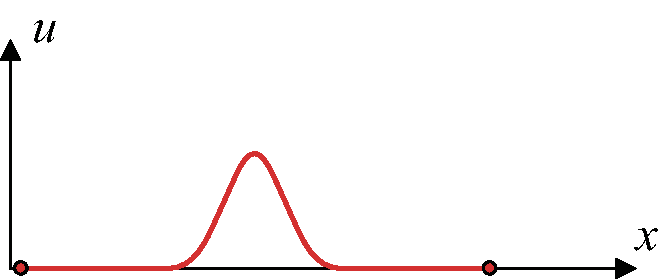
\includegraphics[width=0.35\linewidth]{pic/一维波动非齐次.pdf}
	\caption{一维非齐次波动方程}
	\label{一维波动非齐次}
\end{figure}

\begin{align}
	\begin{cases}
		\, \dfrac{\partial^2 u}{\partial t^2} = a^2 \dfrac{\partial^2 u}{\partial x^2} + f(x,t), &0<x<a,t>0\\[0.5em]
		\, u|_{x = 0} = u_1(t),\, u|_{x = l} = u_2(t), & t>0\\[0.5em]
		\, u|_{t = 0} = \varphi(x),\, \left. \dfrac{\partial u}{\partial x} \right|_{t = 0} = \psi(x), & 0 \le x \le a
	\end{cases}
\end{align}
\begin{enumerate}[\textbf{步骤}1 ]
	\item \textbf{将边界条件齐次化}
	\item \textbf{一分为二}
	\begin{equation*}
		\mbox{一分为二}\, 
		\begin{cases}
			\, \mbox{非齐次项(强迫力)引起的波动过程}\\
			\, \mbox{初始条件引起的波动过程}
		\end{cases}
	\end{equation*}
	\item \textbf{用分离变量法求解方程}
	\begin{equation*}
		\mbox{分离变量法}\, 
		\begin{cases}
			\, \mbox{齐次方程(非零初始条件)的定解问题} \quad \xrightarrow{\scriptsize \,\, \mbox{方法}\,\,} \quad \mbox{常规分离变量法步骤求解}\\
			\, \mbox{非齐次方程(零初始条件)的定解问题}\quad \xrightarrow{\scriptsize \,\, \mbox{方法}\,\,} \quad \mbox{相应齐次
				问题的特征函数展开法求解}
		\end{cases}
	\end{equation*}
	\item \textbf{合二为一}\\
	叠加即得到原问题的解。
\end{enumerate}

\subsection{一维非齐次热传导方程}
\vspace*{-2em}
\begin{align}
	\begin{cases}
		\, \dfrac{\partial u}{\partial t} = a^2 \dfrac{\partial^2 u}{\partial x^2} + f(x,t), &0<x<a,t>0\\[0.5em]
		\, u|_{x = 0} = u_1(t),\, u|_{x = l} = u_2(t), & t>0\\[0.5em]
		\, u|_{t = 0} = \varphi(x), & 0 \le x \le a
	\end{cases}
\end{align}

\begin{figure}[!htb]
	\centering
	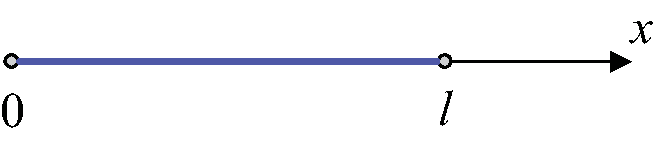
\includegraphics[width=0.35\linewidth]{pic/一维传热非齐次.pdf}
	\caption{一维非齐次传热方程}
	\label{一维传热非齐次}
\end{figure}

\begin{enumerate}[\textbf{步骤}1 ]
	\item \textbf{将边界条件齐次化}
	\item \textbf{一分为二}
	\begin{equation*}
		\mbox{一分为二}\, 
		\begin{cases}
			\, \mbox{非齐次项(热源)引起的传热过程}\\
			\, \mbox{初始条件引起的传热过程}
		\end{cases}
	\end{equation*}
	\item \textbf{用分离变量法求解方程}
	\begin{equation*}
		\mbox{分离变量法}\, 
		\begin{cases}
			\, \mbox{齐次方程(非零初始条件)的定解问题} \quad \xrightarrow{\scriptsize \,\, \mbox{方法}\,\,} \quad \mbox{常规分离变量法步骤求解}\\
			\, \mbox{非齐次方程(零初始条件)的定解问题}\quad \xrightarrow{\scriptsize \,\, \mbox{方法}\,\,} \quad \mbox{相应齐次
				问题的特征函数展开法求解}
		\end{cases}
	\end{equation*}
	\item \textbf{合二为一}\\
	叠加即得到原问题的解。
\end{enumerate}

\subsection{圆域内非齐次Laplace方程}
\vspace*{-2em}
\begin{align}
		\begin{cases}
			\, \dfrac{1}{r}\dfrac{\partial}{\partial r}\left(r \dfrac{\partial u}{\partial r}\right)+\dfrac{1}{r^2}\dfrac{\partial^2 u}{\partial \theta^2} = f_1(r,\theta), & 0<r<a, -\infty < \theta < + \infty\\[0.5em]
			\, u|_{r = a} = f_2(\theta) \, \left|u|_{r = 0}\right| < + \infty, & -\infty < \theta < + \infty\\
			\, u|_{\theta} = u|_{\theta + 2\pi}, & 0<r<a
		\end{cases}
\end{align}

\begin{enumerate}[\textbf{步骤}1 ]
	\item \textbf{坐标变换}\\
	周期性边界条件是齐次的,因此不用边界条件齐次化
	\item \textbf{一分为二}
	\begin{equation*}
		\mbox{一分为二}\, 
		\begin{cases}
			\, \mbox{非齐次项引起的稳态分布}\\
			\, \mbox{非齐次边界条件引起的稳态分布}
		\end{cases}
	\end{equation*}
	\item \textbf{用分离变量法求解方程}
	\begin{equation*}
		\mbox{分离变量法}\, 
		\begin{cases}
			\, \mbox{齐次方程(一组非齐次边界条件)的定解问题} \quad \xrightarrow{\scriptsize \,\, \mbox{方法}\,\,} \quad \mbox{常规分离变量法步骤求解}\\
			\, \mbox{非齐次方程(齐次边界条件)的定解问题}\quad \xrightarrow{\scriptsize \,\, \mbox{方法}\,\,} \quad \mbox{相应齐次
				问题的特征函数展开法求解}
		\end{cases}
	\end{equation*}
	\item \textbf{合二为一}\quad 叠加即得到原问题的解。
\end{enumerate}

\begin{figure}[!htb]
	\centering
	\begin{minipage}{0.45\linewidth}
		\centering
		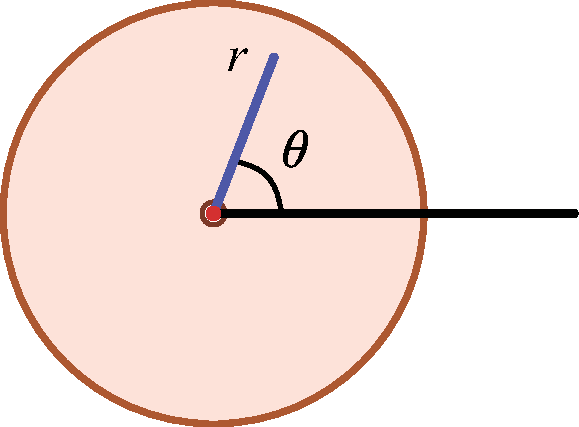
\includegraphics[width=0.5\linewidth]{pic/圆域.pdf}
		\caption{圆域内非齐次Laplace方程}
		\label{圆域}
	\end{minipage}
	\begin{minipage}{0.45\linewidth}
		\centering
		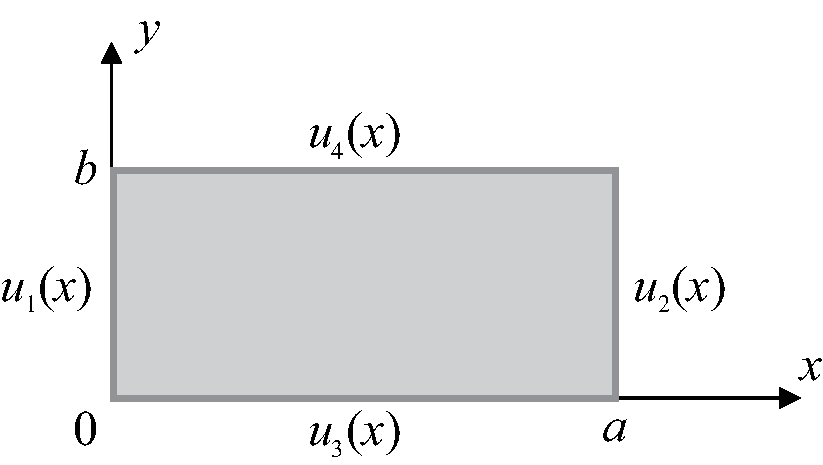
\includegraphics[width=0.743\linewidth]{pic/矩形.pdf}
		\vspace*{-1em}
		\caption{矩形域内非齐次Laplace方程}
		\label{矩形}
	\end{minipage}
\end{figure}
\vspace*{-0.5em}

\subsection{矩形域内非齐次Laplace方程}
\vspace*{-2em}
\begin{align}
	\begin{cases}
		\, \dfrac{\partial^2 u}{\partial x^2} + \dfrac{\partial^2 u}{\partial y^2} = f(x,y), &0 \le x \le a, 0 \le y \le b\\
		\, u|_{x = 0} = u_1(t),\, u|_{x = l} = u_2(t), & 0 \le y \le b\\
		\, u|_{y = 0} = u_3(x),\, u|_{y = b} = u_4(x), & 0 \le x \le a
	\end{cases}
\end{align}
\begin{enumerate}[\textbf{步骤}1 ]
	\item \textbf{将边界条件齐次化}
	\item \textbf{一分为二}
	\begin{equation*}
		\mbox{一分为二}\, 
		\begin{cases}
			\, \mbox{非齐次项引起的稳态分布}\\
			\, \mbox{非齐次边界条件引起的稳态分布}
		\end{cases}
	\end{equation*}
	\item \textbf{用分离变量法求解方程}
	\begin{equation*}
		\mbox{分离变量法}\, 
		\begin{cases}
			\, \mbox{齐次方程(一组非齐次边界条件)的定解问题} \quad \xrightarrow{\scriptsize \,\, \mbox{方法}\,\,} \quad \mbox{常规分离变量法步骤求解}\\
			\, \mbox{非齐次方程(齐次边界条件)的定解问题}\quad \xrightarrow{\scriptsize \,\, \mbox{方法}\,\,} \quad \mbox{相应齐次
				问题的特征函数展开法求解}
		\end{cases}
	\end{equation*}
	\item \textbf{合二为一}\quad 叠加即得到原问题的解。
\end{enumerate}


\begin{figure}
	\subsection{分离变量法解题步骤总结}	
\end{figure}

\begin{figure}[!htb]
	\centering
	\begin{tikzpicture}
		\node (A) [draw, inner sep = 8pt]{列出定解问题};
		\node[diamond] (B) [draw, shape aspect = 4, inner sep = 3pt, below of = A, node distance = 2cm]{坐标轴选取是否恰当?};
		\node (C) [draw, inner sep = 8pt, below of = B, xshift = 4cm, node distance = 1.5cm]{坐标变换};
		\node[diamond] (D) [draw, shape aspect = 4, inner sep = 3pt, below of = B, node distance = 3cm]{边界条件是否齐次?};
		\node (E) [draw, inner sep = 8pt, below of = D, xshift = -4cm, node distance = 1.5cm]{边界条件齐次化};
		\node (F) [draw, inner sep = 8pt, below of = D, node distance = 3cm]{问题的分解};
		\node (H) [draw, inner sep = 8pt, below of = F, node distance = 3cm, xshift = 3.5cm]{\makecell[c]{非齐次方程\\一组齐次边界条件\\一组齐次初始条件}};
		\node (G) [draw, inner sep = 8pt, below of = F, node distance = 3cm, xshift = -3.5cm]{\makecell[c]{齐次方程\\一组齐次边界条件\\一组非齐次初始条件}};
		\node (G1) [draw, inner sep = 8pt, below of = G, node distance = 2.5cm]{常规分离变量法};
		\node (H1) [draw, inner sep = 8pt, below of = H, node distance = 2.5cm]{相应齐次问题的特征函数展开法};
		
		\draw[arrows={-Stealth[scale=0.8]}] (A) -- (B);
		\draw[arrows={-Stealth[scale=0.8]}] (B) -- +(4cm, 0cm)node[midway, above = 0cm]{否} -- (C);
		\draw[arrows={-Stealth[scale=0.8]}] (C) -- +(0cm, -1.5cm) -- (D);
		\draw[arrows={-Stealth[scale=0.8]}] (B) -- (D)node[near start, xshift = -3mm]{是};
		\draw[arrows={-Stealth[scale=0.8]}] (D) -- +(-4cm, 0cm)node[midway, above= 0cm]{否} --(E);
		\draw[arrows={-Stealth[scale=0.8]}] (E) -- +(0cm, -1.5cm) -- (F);
		\draw[arrows={-Stealth[scale=0.8]}] (D) -- (F)node[near start, xshift = -3mm]{是};
		\draw[arrows={-Stealth[scale=0.8]}] (F) -- +(0cm, -1cm) --+ (3.5cm, -1cm) -- (H);
		\draw[arrows={-Stealth[scale=0.8]}] (F) -- +(0cm, -1cm) --+ (-3.5cm, -1cm) -- (G);
		\draw[arrows={-Stealth[scale=0.8]}] (G) -- (G1);
		\draw[arrows={-Stealth[scale=0.8]}] (H) -- (H1);
	\end{tikzpicture}
	\caption{一般分离变量法解题步骤}
	\label{分离变量法S}
\end{figure}


\begin{figure}[!htb]
	\centering
	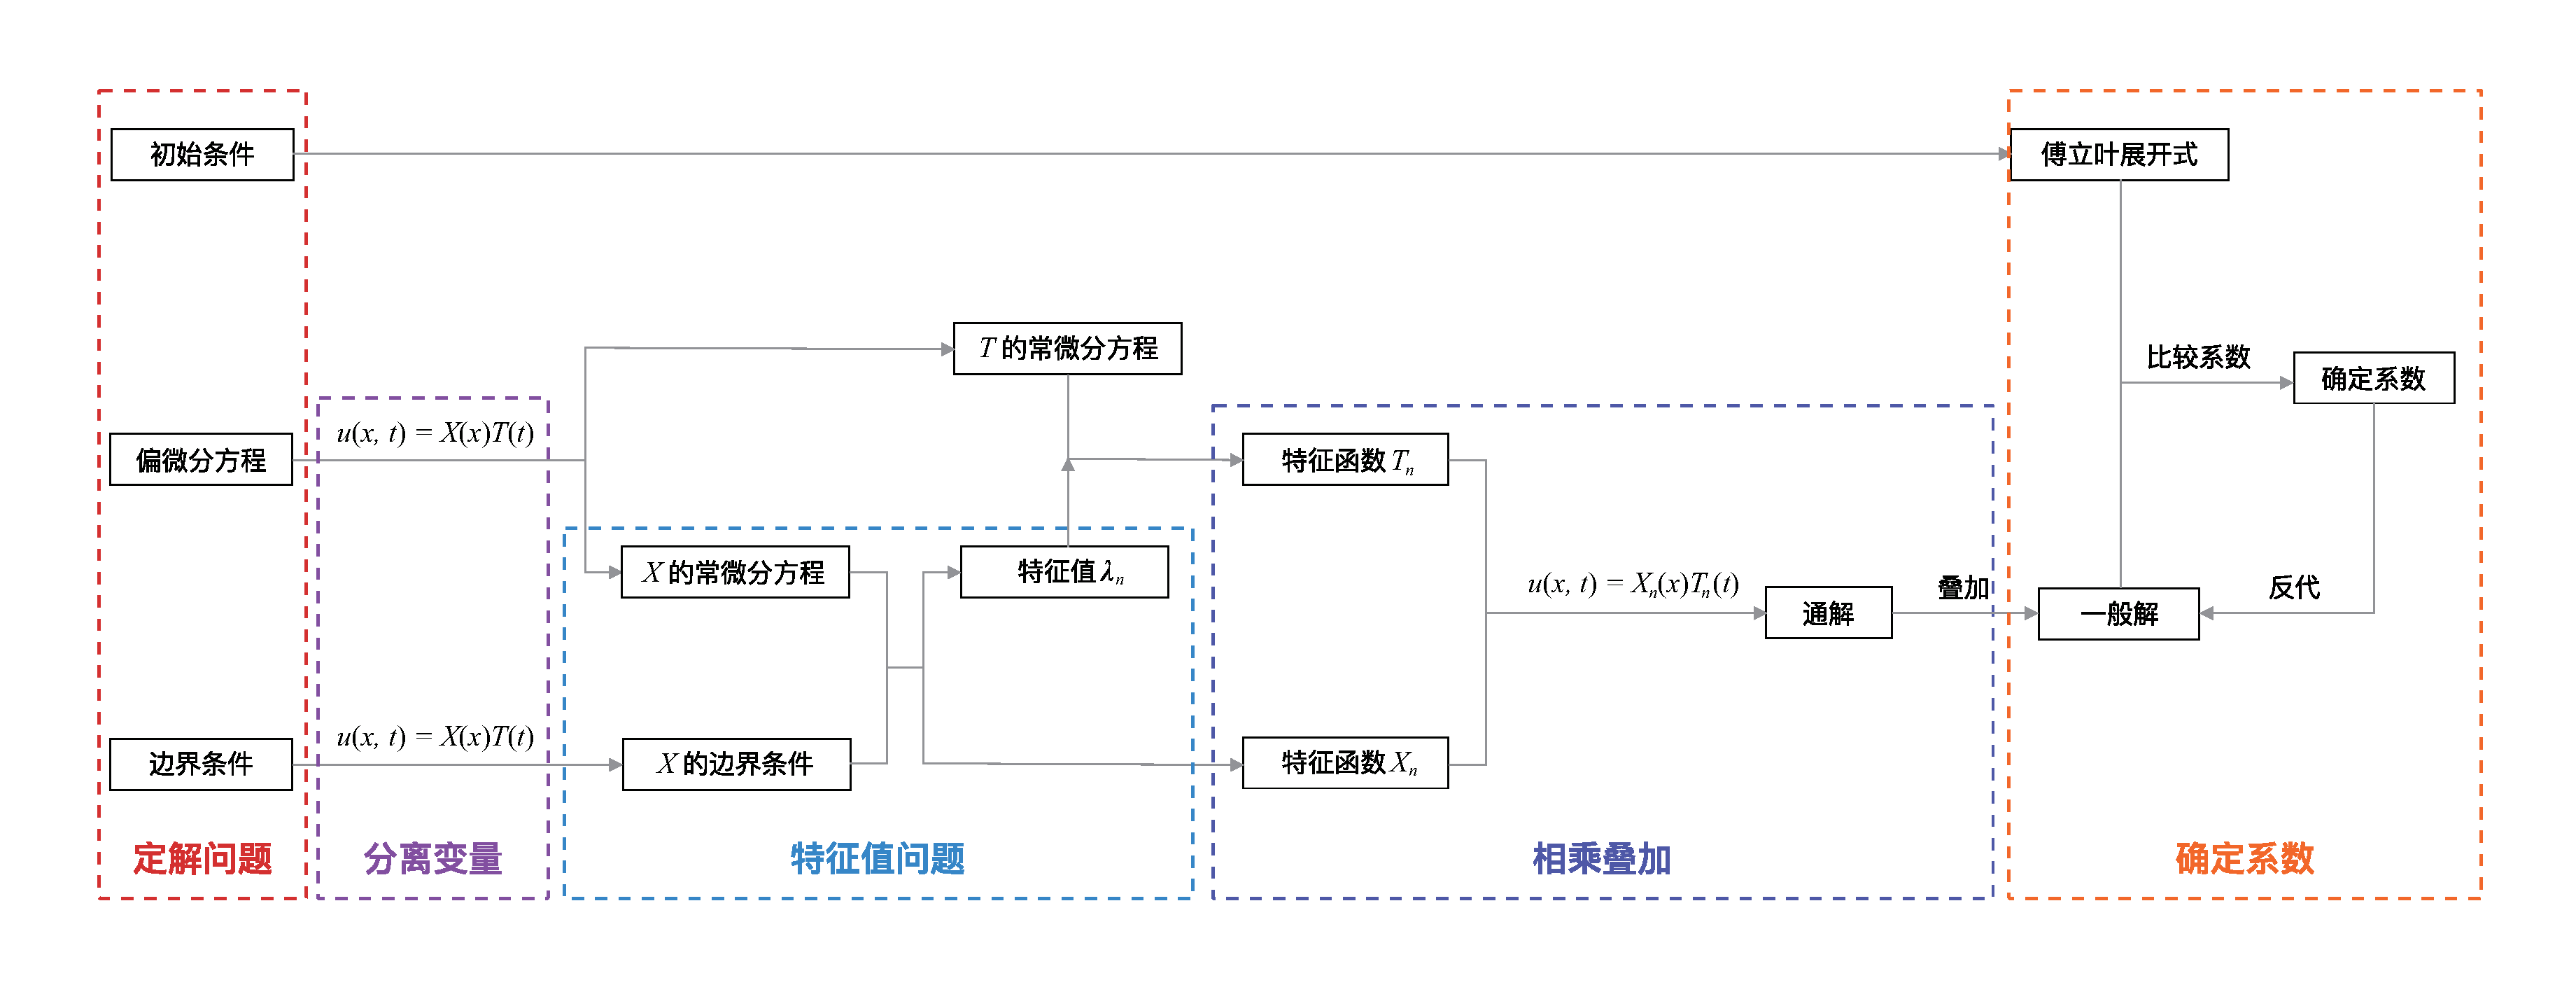
\includegraphics[width=\linewidth]{pic/分离变量.pdf}
	\caption{常规分离变量法步骤}
	\label{分离变量S.1}
\end{figure}

\begin{figure}[!htb]
	\centering
	\begin{tikzpicture}
		\node (A) [draw, inner sep = 5pt]{求相应齐次问题的特征函数$X_n(x)$};
		\node (B) [draw, inner sep = 5pt, below of = A, node distance = 1.5cm]{解和非齐次项表示成特征函数的展开};
		\node (C1) [draw, inner sep = 5pt, below of = B, node distance = 3cm,xshift = -3.5cm]{$\displaystyle V(x,t) = \sum_{n = 1}^\infty v_n(t) X_n(x)$};
		\node (C2) [draw, inner sep = 5pt, below of = B, node distance = 3cm, xshift = 3.5cm]{$\displaystyle f(x,t) = \sum_{n = 1}^\infty f_n(t) X_n(x)$};
		\node (D2) [draw, inner sep = 5pt, below of = C2, node distance = 1.5cm]{根据特征函数正交性,获得系数$f_n(t)$};
		\node (E) [draw, inner sep = 5pt, below of = B, node distance = 6cm]{代入偏微分方程和初始条件,获得$v_n(t)$的常微分方程和定解条件};
		\node (F) [draw, inner sep = 5pt, below of = E, node distance = 1.5cm]{求解得$v_n(t)$,代回展开式得$V(x,t)$};
		
		\draw[arrows={-Stealth[scale=0.8]}] (A) -- (B);
		\draw[arrows={-Stealth[scale=0.8]}] (B) -- +(0cm, -1.5cm) -- +(-3.5cm,-1.5cm) -- (C1);
		\draw[arrows={-Stealth[scale=0.8]}] (B) -- +(0cm,-1.5cm) -- +(3.5cm,-1.5cm) -- (C2);
		\draw[arrows={-Stealth[scale=0.8]}] (C1) -- + (0cm, -2.25cm) -- +(3.5cm, -2.25cm) -- (E);
		\draw[arrows={-Stealth[scale=0.8]}] (C2) -- (D2);
		\draw[arrows={-Stealth[scale=0.8]}] (D2) -- +(0cm, -0.75cm) -- +(-3.5cm,-0.75cm) -- (E);
		\draw[arrows={-Stealth[scale=0.8]}] (E) -- (F);
	\end{tikzpicture}
	\caption{相应齐次问题的特征函数展开法}
	\label{分离变量法S.2}
\end{figure}


\examples 研究均匀细杆的导热问题,其中均匀细杆中有一个与温度$u$成正比的负热源,求下列定解问题
\begin{align}
	\begin{cases}
		\, \dfrac{\partial u}{\partial t} = a^2 \dfrac{\partial^2 u}{\partial x^2} - b^2 u, & 0<x<l,t>0\\[0.5em]
		\, \left. \dfrac{\partial u}{\partial x}\right|_{x = 0} = 0, u|_{x = l} = 0, &t > 0\\[0.5em]
		\, u|_{t = 0} = \dfrac{u_1}{l^2}x^2, &0<x<l
	\end{cases}
\end{align}
思路
\begin{itemize}
	\item 边界形状简单,无需坐标变换
	\item 边界条件非齐次,需要齐次化边界条件
\end{itemize}

\solve 
\begin{enumerate}[{\textbf{步骤}}1 ]
	\item  \textbf{边界条件齐次化}\\
	\hspace*{2em} 将边界条件齐次化,令
	\begin{align}
		u(x,t) = V(x, t) + u_1
	\end{align}
	代入原定解问题,可得
	\begin{align}
		\begin{cases}
			\, \dfrac{\partial V}{\partial t} = a^2 \dfrac{\partial^2 V}{\partial x^2} - b^2 V - b^2u_1, & 0<x<l,t>0\\[0.5em]
			\, \left. \dfrac{\partial V}{\partial x}\right|_{x = 0} = 0, V|_{x = l} = 0, &t > 0\\[0.5em]
			\, V|_{t = 0} = \dfrac{u_1}{l^2}x^2 - u_1, &0\le x\le l
		\end{cases}
	\end{align}
	
	\item \textbf{一分为二}\\
	由于方程是非齐次的且边界条件也是非齐次的,所以需要将方程进一步分解为两个方程,引入变量拆分:
	\begin{align}
		V(x,t) = v(x,t) + g(x,t)
	\end{align}
	
	\begin{itemize}
		\item 边界条件不为0的自由传热方程(初始非0温度分布的贡献)
		\begin{align}
			\begin{cases}
				\, \dfrac{\partial v}{\partial t} = a^2 \dfrac{\partial^2 v}{\partial x^2} - b^2 v, &0<x<l,t>0 \\[0.5em]
				\, \left. \dfrac{\partial v}{\partial x} \right|_{x = 0} = 0, v|_{x = l} = u_1, &t>0\\[0.5em]
				\, v|_{t = 0} = \dfrac{u_1}{l^2}x^2 - u_1, &0 \le x \le l
			\end{cases}
		\end{align}
		\begin{enumerate}[\textbf{第} 1 \textbf{步} ]
			\item \textbf{分离变量}\\
			设$v(x, t) = X(x)T(t)$,代入齐次方程,得到
			\begin{align}
				\begin{aligned}
					& X'' + \beta X = 0\\
					& X'(0) = X(l) = 0
				\end{aligned}
				\quad \quad \quad 
				T' + (b^2 + a^2 \beta^2)T = 0
			\end{align}
			
			\item \textbf{解特征值问题}\\
			对$\beta $进行分类讨论,最后得到
			\begin{align}
				& \beta^2 = \dfrac{(2n+1)^2\pi^2}{4l^2}\quad (n = 0,1,2,\cdots)\\
				& X_n(x) = B_n \cos \left[\dfrac{(2n+1)\pi}{2l}x\right]
			\end{align}
			
			\item \textbf{解另一方程}\\
			将特征值代入关于$T(t)$的微分方程,可以解得
			\begin{align}
				T_n(t) = C_n \exp \left \lbrace\left[-b^2 - \dfrac{(2n+1)^2\pi^2 a^2}{4l^2}\right]t\right\rbrace
			\end{align}
			
			\item \textbf{相乘叠加得一般解}\\
			相乘叠加,得
			\begin{align}
				v(x,t) = \sum_{n = 0}^{\infty} C_n \exp \left \lbrace\left[-b^2 - \dfrac{(2n+1)^2\pi^2 a^2}{4l^2}\right]t\right\rbrace \cos \left[\dfrac{(2n+1)\pi}{2l}x\right]
			\end{align}
			
			\item \textbf{确定叠加系数}\\
			由特征值卷积为0的性质,可得
			\begin{align}
				v|_{t = 0} &= v(x, 0) =\sum_{n = 0}^{\infty} C_n \cos\left[\dfrac{(2n+1)\pi}{2l}x\right] =  \dfrac{u_1}{l^2}x^2 - u_1\\[0.5em]
				C_n &= \dfrac{\displaystyle \int_0^l \left(\dfrac{u_1}{l^2}x^2 - u_1\right)\cos \left[\dfrac{(2n+1)\pi}{2l}x\right]  \, \d x}{ \displaystyle \int_0^l \cos^2 \left[\dfrac{(2n+1)\pi}{2l} x\right] \, \d x}\\[0.5em]
				& = \dfrac{2}{l} \int_0^l \left(\dfrac{u_1}{l^2}x^2 - u_1\right) \cos \left[\dfrac{(2n+1)\pi}{2l}x\right] \, \d x \notag \\[0.5em]
				& = \dfrac{2}{l} \cdot \left[- \dfrac{16 u_1 l}{(2n + 1)^3\pi^3} \sin \left(\dfrac{(2n + 1)\pi}{2}\right)\right]\notag \\[0.5em]
				& = (-1)^{n + 1} \dfrac{32 u_1}{(2n + 1)^3 \pi^3}
			\end{align}
		\end{enumerate}
		所以,得到最终结果为
		\begin{align}
			v(x, t) = \dfrac{32 u_1}{\pi^3} \exp(-b^2 t) \sum_{n = 0}^{\infty} \dfrac{(-1)^{n+1}}{(2n+1)^3} \exp \left[- \dfrac{(2n+1)^2\pi^2 a^2}{4l^2} t\right] \cos \left[ \dfrac{(2n+1)\pi}{2} x\right]
		\end{align}
		\vspace*{1em}
	
		\item 含有热源初始条件为0的受干扰的传热方程(恒定热源$-b^2u_1$的贡献)
		\begin{align}
			\begin{cases}
				\, \dfrac{\partial g}{\partial t} = a^2 \dfrac{\partial^2 g}{\partial x^2} - b^2 g - b^2 u_1, &0<x<l,t>0 \\[0.5em]
				\, \left. \dfrac{\partial g}{\partial x} \right|_{x = 0} = 0, g|_{x = l} = 0, &t>0\\[0.5em]
				\, g|_{t = 0} = 0, &0 \le x \le l
			\end{cases}
		\end{align}
		\begin{enumerate}[\textbf{步骤} 1 ]
			\item \textbf{按相应齐次问题的特征函数展开}\\
			将$g(x,t)$及其方程中的非齐次项均按相应齐次问题的特征函数展开
			\begin{align}
				&g(x,t) = \sum_{n = 0}^{\infty} g_n(t)\cos \left[\dfrac{(2n+1)\pi}{2} x\right]\\[0.5em]
				&-b^2u_1 = \sum_{n = 0}^{\infty} f_n\cos \left[\dfrac{(2n+1)\pi}{2} x\right]
			\end{align}
			
			\item \textbf{由特征函数正交性确定非齐次项叠加系数}
			\begin{align}
				g_n = \dfrac{\displaystyle \int_0^l -b^2 u_1\cos \left[\dfrac{(2n+1)\pi}{2l}x\right]  \, \d x}{ \displaystyle \int_0^l \cos^2 \left[\dfrac{(2n+1)\pi}{2l} x\right] \, \d x} = (-1)^{n+1} \dfrac{4 b^2 u_1}{(2n+1) \pi}
			\end{align}
			
			\item \textbf{将展开式代入方程和初始条件得常微分方程}
			\begin{align}
				\begin{cases}
					\, g_n'(t) + \left[\dfrac{(2n+1)^2\pi^2}{4l^2} + b^2\right] g_n(t) = (-1)^{n+1} \dfrac{4 b^2 u_1}{(2n+1) \pi} \\[0.5em]
					\, g_n(0) = 0
				\end{cases}
			\end{align}
			
			\item \textbf{Laplace变换求解常微分方程}\\[0.5em]
			令常数$A = \dfrac{(2n+1)^2\pi^2}{4l^2} + b^2, B = (-1)^{n+1} \dfrac{4 b^2 u_1}{(2n+1) \pi}$,并记$\mathcal{L}\big[g_n(t)\big] = G_n(s)$。\\[0.5em]
			对常微分方程取Laplace变换,得
			\begin{align}
				s G_n(s) + A G_n(s) = \dfrac{B}{s} \quad \Rightarrow \quad G_n(s) = \dfrac{B}{s(s + A)} = \dfrac{B}{A - 1} \left(\dfrac{1}{s} - \dfrac{1}{s + A}\right)
			\end{align}
			取逆变换,得
			\begin{align}
				g_n(t) &= \mathcal{L}^{-1}\big[G_n(s)\big] = \dfrac{B}{A-1}\left(1 - \e^{-At}\right) \notag \\[0.5em]
				& = \dfrac{(-1)^n 16b^2 u_1l^2}{(2n+1)\pi \big[4b^2l^2 + (2n + 1)^2\pi^2 a^2\big]}\left\{ \exp \left[- \dfrac{(2n+1)^2\pi^2a^2 + 4l^2b^2}{4l^2} t\right] - 1\right\}
			\end{align}
		
			\item \textbf{代入特征函数叠加得一般解}
		\end{enumerate}
	\end{itemize}
	\vspace*{-0.5em}
	\begin{align}
		g(x,t) = \dfrac{16b^2 u_1l^2}{\pi}\sum_{n = 0}^{\infty} \dfrac{(-1)^n}{(2n+1) \big[4b^2l^2 + (2n + 1)^2\pi^2 a^2\big]}\left\{ \exp \left[- \dfrac{(2n+1)^2\pi^2a^2 + 4l^2b^2}{4l^2} t\right] - 1\right\}\cos \left[\dfrac{(2n+1)\pi}{2} x\right]
	\end{align}
	
	\item \textbf{合二为一}
	\begin{equation}
		\begin{split}
			u(x, t) &= V(x, t) + u_1 = v(x, t) + g(x, t) + u_1\\[0.5em]
			& =  \dfrac{16b^2 u_1l^2}{\pi}\sum_{n = 0}^{\infty} \dfrac{(-1)^n}{(2n+1) \big[4b^2l^2 + (2n + 1)^2\pi^2 a^2\big]}\left\{ \exp \left[- \dfrac{(2n+1)^2\pi^2a^2 + 4l^2b^2}{4l^2} t\right] - 1\right\}\cos \left[\dfrac{(2n+1)\pi}{2} x\right] \\[0.5em]
			& + \dfrac{32 u_1}{\pi^3} \exp(-b^2 t) \sum_{n = 0}^{\infty} \dfrac{(-1)^{n+1}}{(2n+1)^3} \exp \left[- \dfrac{(2n+1)^2\pi^2 a^2}{4l^2} t\right] \cos \left[ \dfrac{(2n+1)\pi}{2} x\right] + u_1
		\end{split}
	\end{equation}
\end{enumerate}

\renewcommand{\thempfootnote}{\arabic{mpfootnote}}
\warn[
分离变量法的适用条件\vspace*{-0.5em}
{
\begin{enumerate}
	\item 方程和定解条件都是线性的\vspace*{-0.5em}
	\item 边界形状规则 \footnote[1]{边界在某种坐标系中能用若干个仅含有一个坐标变量的方程表示,即边界与坐标轴垂直}\vspace*{-0.5em}
	\item 有限域内的定解问题\vspace*{0.5em}
\end{enumerate}
}
]






















 






